%
% Chapter 2
%
% Systems vaccinology-style paper.

% The one central and memorable contribution of the paper.
\chapter{Transcriptomic response to influenza A (H1N1)pdm09 vaccine (Pandemrix)}

% Chapter 2 HIRD sysvacc abstract

\section{Introduction}

\subsection{Influenza A (H1N1)pdm09 and Pandemrix}

\begin{outline}

% Intro to the virus (Characteristics of Swine-Origin 2009 A(H1N1), DOI: 10.1126/science.1176225)
\1 Basic H1N1 biology
    \2 structure and life cycle.
    \2 relationship to other (seasonal) influenza viruses.

\1 The 2009 outbreak.
    % http://europepmc.org/article/PMC/3224079
    \2 origins; timeline

\1 Vaccine development process in response to the outbreak
    % \url{https://www.ema.europa.eu/en/human-regulatory/overview/public-health-threats/pandemic-influenza/2009-h1n1-influenza-pandemic/medicines-authorised-during-pandemic}
    \2 Pandemrix was one of several vaccines licensed
    % \url{https://www.ncbi.nlm.nih.gov/pmc/articles/PMC3224079/}
    \2 Efficacy, dosing: \enquote{...a single dose of monovalent 2009 H1N1 vaccine was recommended in adults, but young children were recommended to receive 2 doses (reviewed by [3••]). It is likely that a single dose was sufficient to induce immunity in adults because prior exposure to seasonal H1N1 viruses had immunologically primed the population.}
    % "Seasonal influenza vaccine provides priming for A/H1N1 immunization." \url{https://www.ncbi.nlm.nih.gov/pubmed/20371459}
    % Demonstration in a mouse model: \url{https://www.ncbi.nlm.nih.gov/pmc/articles/PMC3024675/}
    \2 Inclusion of H1N1 strains into seasonal vaccines
        % Sobolev sampled in March 2010 to August 2011
        \3 Later cohorts may have recall response to H1N1 from seasonal vaccination.

\end{outline}

\subsection{Systems vaccinology of influenza vaccines}

\begin{outline}

\1 Review influenza vaccine specific sysvacc papers (e.g. Nakaya's papers)
    \2 inclu. prevaccination signatures paper

\end{outline}

\subsection{The \glsfmtfull{HIRD} study}

\begin{outline}

% Summarise sobolev
\1 Systems vaccinology of Pandemrix vaccine: Sobolev et al. 2016

    \2 Sobolev et al 2016 evaluated transcriptomic, cellular, antibody and adverse events after AS03-adjuvanted Pandemrix vaccination.
        \3 Myeloid response similar to other unadjuvanted flu vaccines
        % \enquote{biggest fold-change was in interferon-γ (IFN-γ), a cytokine associated with type 1 helper T cells (TH1 cells), cytolytic T cells, γδ T cells, natural killer T (NKT) cells, NK cells and type 1 innate lymphoid cells (Fig. 1e).}
        \3 Early lymphoid response unlike other unadjuvanted vaccines
            \4 Knowns about the immune response to AS03
        \3 Non responders had \enquote{reduced expression of genes associated with plasma cell development and antibody production at day 7}
        \3 No consensus NR signatures at earlier timepoints day 0 or day 1 \enquote{many routes to failure}. One reason is variable baseline titres leading to variable trajectories of NR.

\end{outline}

\subsection{Chapter summary}

\begin{outline}

    \1 Rationale for our study
        \2 Sobolev uses array transcriptomic data for a subset of individuals; we use RNAseq data for a larger number of individuals, which allows us to look at a larger number of genomic features, and conduct a meta-analysis.
        \2 Instead of the binary definition for responder/NR used by Sobolev, we use a continuous response measure, for increased power. This also lets us normalise for baseline titre and combine HAI and microneutralization assay values.
            \3 can we find consensus, and importantly prevaccination signatures of response?
    \1 Main conclusions
        \2 The overall pattern of innate response at d1, adaptive response at d7, agrees with Sobolev.
        \2 Based on our continuous Ab phenotype, we find consensus response signatures
            \3 plasma cells and inflammatory response overall
            \3 at each timepoint, d0, d1, d7 ... TODO
                \4 Compare the d7 split to Sobolev TODO 

\end{outline}

\section{Methods}

\subsection{Pre-existing \glsfmtshort{HIRD} study data and additional sampling}

Sample demographics: age, sex, self-reported ethnicity

\begin{figure}
    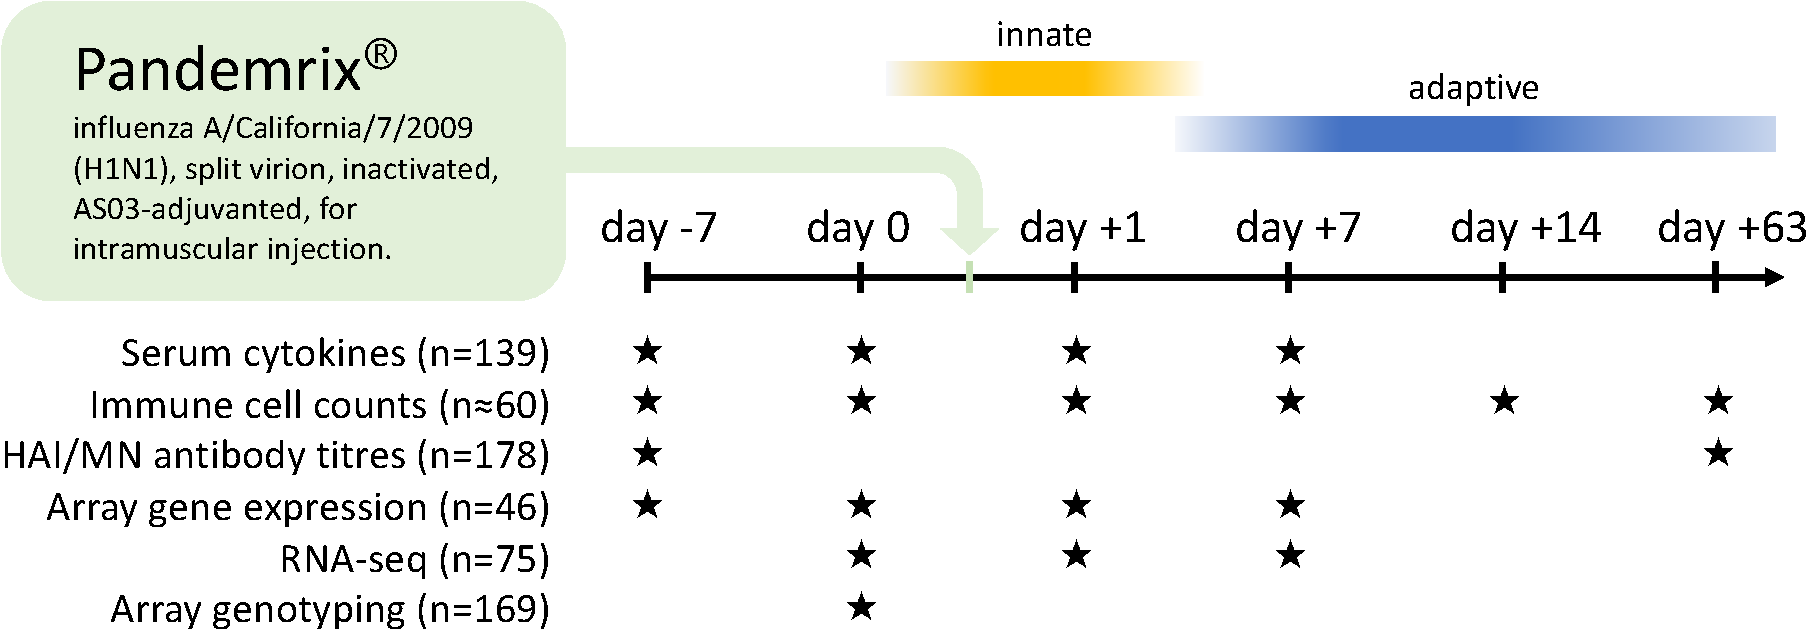
\includegraphics[width=1.0\textwidth]{./mainmatter/figures/chapter_02/graphics/hird_design-crop.pdf}
    \caption{Data types, timepoints, and sample sizes. Individuals were vaccinated after day 0 sampling. Vaccine-induced antibodies measured by \gls{HAI} and \gls{MN} assays. Array and \gls{RNAseq} gene expression measured in the \gls{PBMC} compartment.}
    \label{fig:hird_design}
\end{figure}

\subsection{Genotype data generation}

DNA extraction; genotyping array

\subsection{Genotype data preprocessing}

% 1.	QC
% 2.	Online imputation service to phase and impute chr 1-22 and X
% 2.1.	Phase with Eagle v2.4 (version in imputation logs.tar.gz)
% 2.2.	Impute with PBWT 3.1-v3.1-2-gbf6ebe2+htslib-1.3.2-199-gec1d68e-dirty (version in vcf header)
% 2.2.1.	Reference fa is human_g1k_v37.fasta (1000 genomes)
% 2.2.2.	X chrom is done in 3 chunks
% 2.2.2.1.	X:1-2699520: impute against reference resources/refs/imputation/hrc.r1.1/pbwt/HRC.r1-1.GRCh37.chrX_PAR1.shapeit3.mac5.aa.genotypes
% 2.2.2.2.	X:2699521-154931043: impute against reference resources/refs/imputation/hrc.r1.1/pbwt/HRC.r1-1.GRCh37.chrX_nonPAR.shapeit3.mac5.aa.genotypes
% 2.2.2.3.	X:154931044-155270560: impute against reference resources/refs/imputation/hrc.r1.1/pbwt/HRC.r1-1.GRCh37.chrX_PAR2.shapeit3.mac5.aa.genotypes
% 3.	Liftover with crossmap
% 4.	Filtering
% 4.1.	BCFTOOLS_INCLUDE="MAF>$MAF_THRESH & F_MISSING<0.05 & FILTER==\"PASS\" & INFO/INFO>0.4"
% 4.2.	Use MAF thresholds 0.05, 0.10, 0.20
% Impute PCs
Sample and marker QC; phasing and imputation; post-imputation filters; PC projection; PC imputation

\begin{figure}
    \includegraphics[width=1.0\textwidth,page=2]{./mainmatter/figures/chapter_02/coreex_eQTLflu_20171204.gencall.smajor.impute_sex.qc2.pdf}
    \caption{Sample filters for missingness vs heterozygosity rate.}
\end{figure}

\begin{figure}
    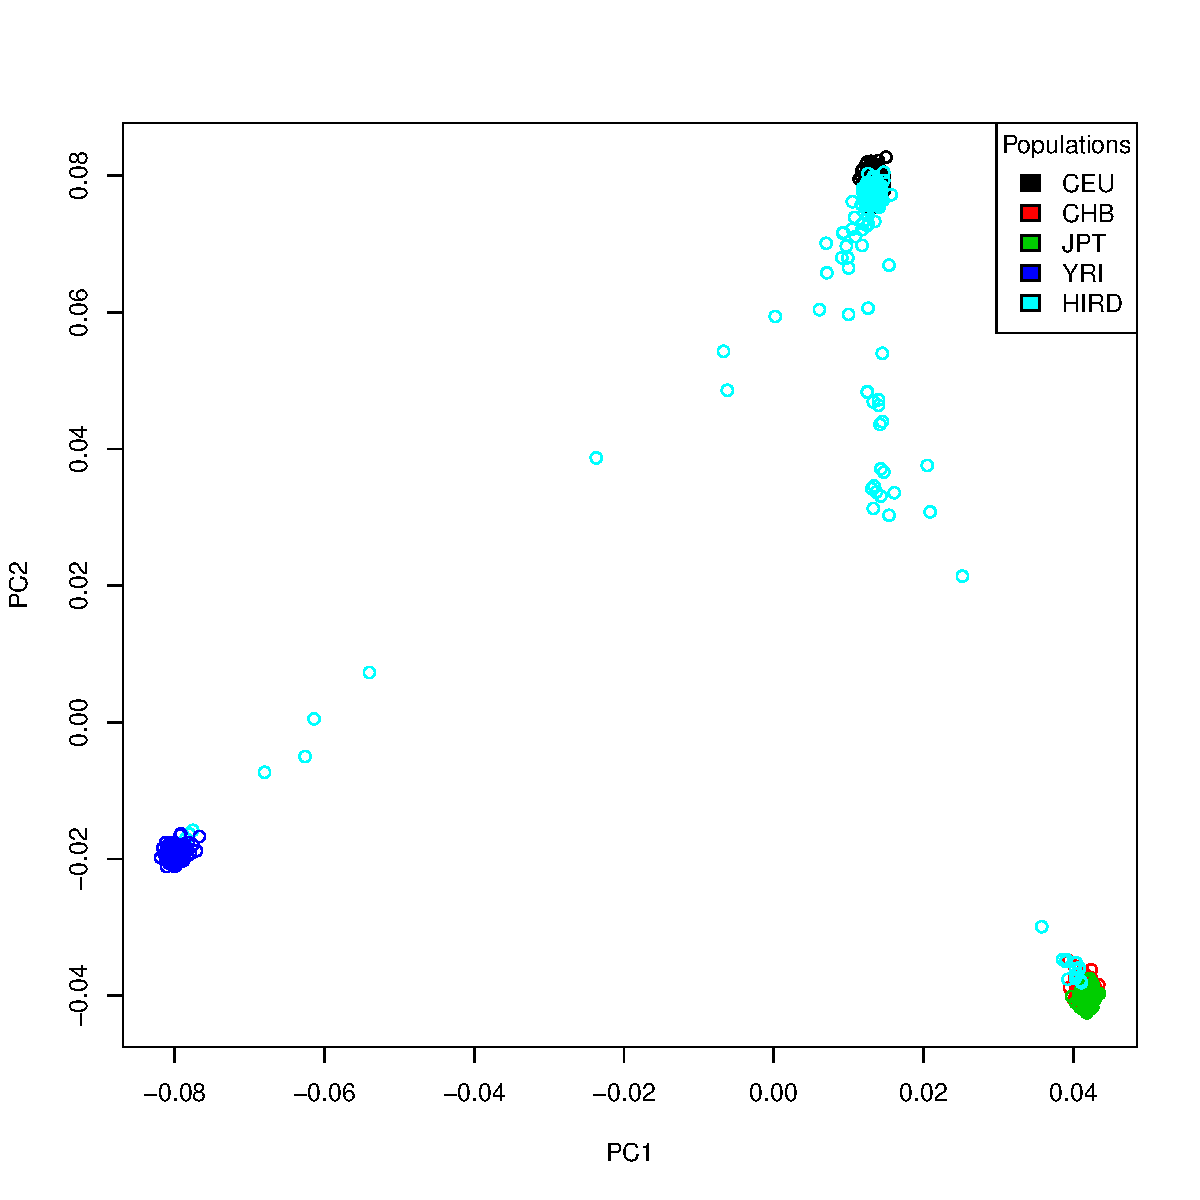
\includegraphics[width=1.0\textwidth]{./mainmatter/figures/chapter_02/coreex_eQTLflu_20171204.gencall.smajor.impute_sex.qc3.pruned.hapmap_merged.flipped.pca.evec.pdf}
    \caption{Samples projected onto HapMap PC axes.}
\end{figure}

\subsection{RNA-seq data generation}

Do we have enough reads for RNAseq analysis? \url{https://www.ncbi.nlm.nih.gov/pubmed/24434847} and doi:10.1093/bioinformatics/btt688

Summing tech reps: sum of poison is poisson, average is not: https://www.biostars.org/p/304552/

\subsection{RNA-seq data preprocessing}

% From .cram headers:
% 1.	The NextSeq, HiSeq, and NovaSeq Sequencing Systems generate raw data files in binary base call (BCL) format.
% 1.1.	HiSeq Sequencing Control Software (SCS), version HD 3.4.0.38, used for basecalling
% 2.	biobambam2/bamadapterfind: bamdapterfind scans a BAM file for contaminations by sequencing adapters.
% 3.	bambi decode: decode a multiplexed bam file
% 4.	bwa sampe (alignment using BWA-backtrack): alignment to phiX, which is then merged with the original bam
% 5.	pb_calibration/spatial_filter: Identify regions with spatially correlated errors e.g. bubbles, (from aligned BAM files where the read name can be parsed for spatial location) and allow filtering out or marking of the BAM fail bit for reads in those regions.
% 6.	Alignment with tophat 2.0.14
% 6.1.	 --keep-fasta-order --no-sort-bam --output-dir tophat_out_24165_1#10 --mate-inner-dist 100 --num-threads=8 --library-type=fr-firststrand --no-coverage-search --microexon-search --transcriptome-index=/lustre/scratch117/core/sciops_repository/transcriptomes/Homo_sapiens/ensembl_83_transcriptome/GRCh38_15_plus_hs38d1/tophat2/GRCh38_15_plus_hs38d1.known/lustre/scratch117/core/sciops_repository/references/Homo_sapiens/GRCh38_15_plus_hs38d1/all/bowtie2/Homo_sapiens.GRCh38_15_plus_hs38d1.fa
% 7.	Some sort of duplicate marking and filtering (?) using some combination of:
% 7.1.	biobambam/bamsormadup: parallel sorting and duplicate marking
% 7.2.	uk.ac.sanger.npg.picard.AlignmentFilter
% 7.3.	biobambam/bamstreamingmarkduplicates
% 8.	Write .cram files using scramble (cram is a reference-based compression)
% 8.1.	/lustre/scratch117/core/sciops_repository/references/Homo_sapiens/GRCh38_15_plus_hs38d1/all/fasta/Homo_sapiens.GRCh38_15_plus_hs38d1.fa
% 9.	NOTE: Note lots of intermediate biobambam 2.0.76 and scramble processing steps, not all are listed.

\begin{outline}
QC
\1 fastqc (sequence quality, GC content, length, duplication, overrepresented sequences incl adapters)
\1 qualimap
\1 salmon qc
\end{outline}

\begin{figure}
    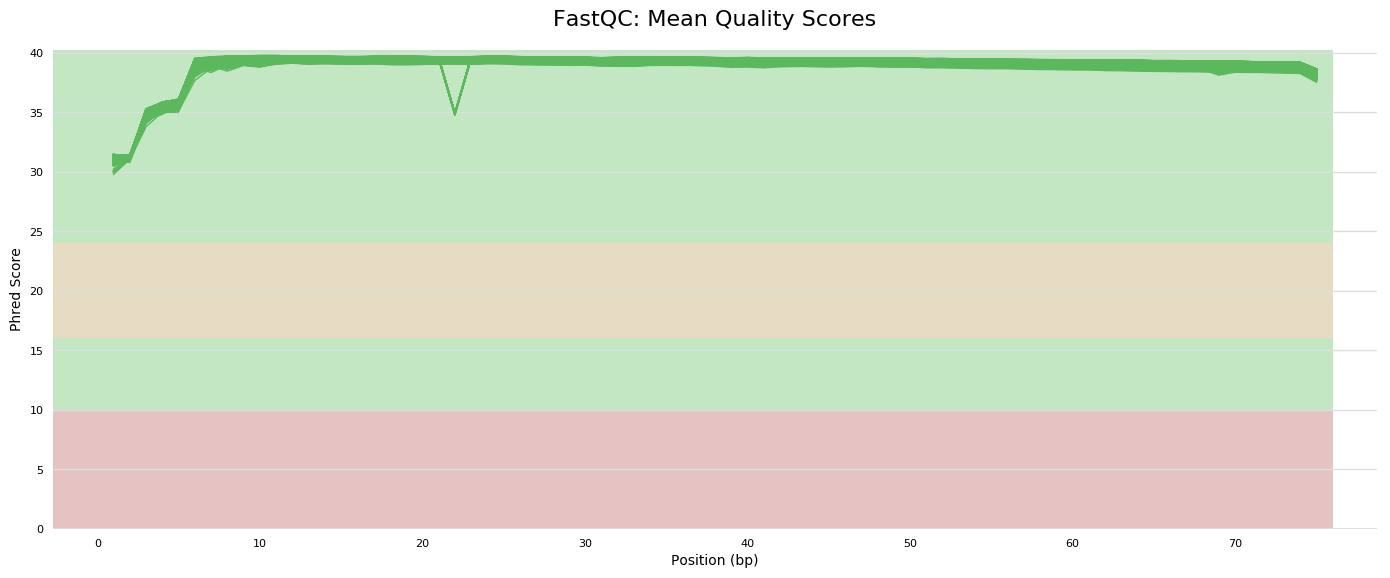
\includegraphics[width=1.0\textwidth]{./mainmatter/figures/chapter_02/fastqc_Sequence Quality Histograms.png}
    \caption{The mean quality value across each base position in the read.}
    \label{fig:fastqc_sequenceQualityHistogram}
\end{figure}

% 1.	Quantification (Salmon --libType ISR, which is equiv to TopHat -fr-firststrand with paired end data)
% 1.1.	Used index /lustre/scratch117/core/sciops_repository/transcriptomes/Homo_sapiens/ensembl_83_transcriptome/GRCh38_15_plus_hs38
% 1.1.1.	This is GRCh38.p5, Dec 2017, v83; with additional hs38d1: Decoy version 1 for GRCh38
% 1.1.2.	Contains ENST transcript ids
% 1.2.	Output quantifies transcripts in terms of: TPM — This is salmon’s estimate of the relative abundance of this transcript in units of Transcripts Per Million (TPM). TPM is the recommended relative abundance measure to use for downstream analysis.
% 1.2.1.	https://haroldpimentel.wordpress.com/2014/05/08/what-the-fpkm-a-review-rna-seq-expression-units/ TPM = (count/effectiveLength) / sumOverAllTranscripts(count/effectiveLength)
% 1.3.	Note Salmon also takes into account: EffectiveLength — This is the computed effective length of the target transcript. It takes into account all factors being modeled that will effect the probability of sampling fragments from this transcript, including the fragment length distribution and sequence-specific and gc-fragment bias (if they are being modeled).
% 2.	Gene-level regeneration of counts (tximport)
% 2.1.	“generate estimated counts using abundance estimates scaled up to library size (scaledTPM)”
% 2.1.1.	Note, we do not scale for gene length, that would be lengthScaledTPM. Hence the generated counts remain length-corrected.
% 2.2.	Summarizes using a mapping of ENST to ENSG, generated from /lustre/scratch117/core/sciops_repository/transcriptomes/Homo_sapiens/ensembl_83_transcriptome/GRCh38_15_plus_hs38d1/gtf/ensembl_83_transcriptome-GRCh38_15_plus_hs38d1.gtf
% 2.3.	Counts from all lanes of a sample are summed
% 3.	GC bias, length bias, mappability
% 3.1.	Length bias only affects RNAseq: somewhat alleviated by Salmon using effective length
% 3.2.	GC bias affects both technologies: somewhat alleviated by Salmon using effective length (see the salmon paper)
% 3.3.	Mappability has not been considered

Quantification

% 5.	Pre-process RNA-seq expression data
% 5.1.	Pull in tximport counts
% 5.1.1.	60675 loci, 223 samples
% 5.2.	Add gene annotation based on EnsDb.Hsapiens.v86
% 5.3.	Low-count filtering (>0.5 CPM in 10% of 223 samples i.e. 22 samples)
% 5.3.1.	29138 loci, 223 samples
% 5.4.	Remove globin genes and short non-coding RNAs
% 5.4.1.	Human globins: https://en.wikipedia.org/wiki/Globin#Examples
% 5.4.2.	Short non-coding GENEBIOTYPES: https://www.gencodegenes.org/pages/biotypes.html
% 5.4.3.	26275 loci, 223 samples
% 5.5.	NOTE: we have not yet removed GENEBIOTYPE=NA. These may be retired ids.
% 5.6.	Between-sample normalization of library size: Trimmed mean of M-values (TMM)
% Selecting between-sample RNA-Seq normalization methods from the perspective of their assumptions https://www.ncbi.nlm.nih.gov/pmc/articles/PMC6171491/
% 5.6.1.	edgeR::calcNormFactors generates norm.factors for each sample

Filtering
\begin{figure}
    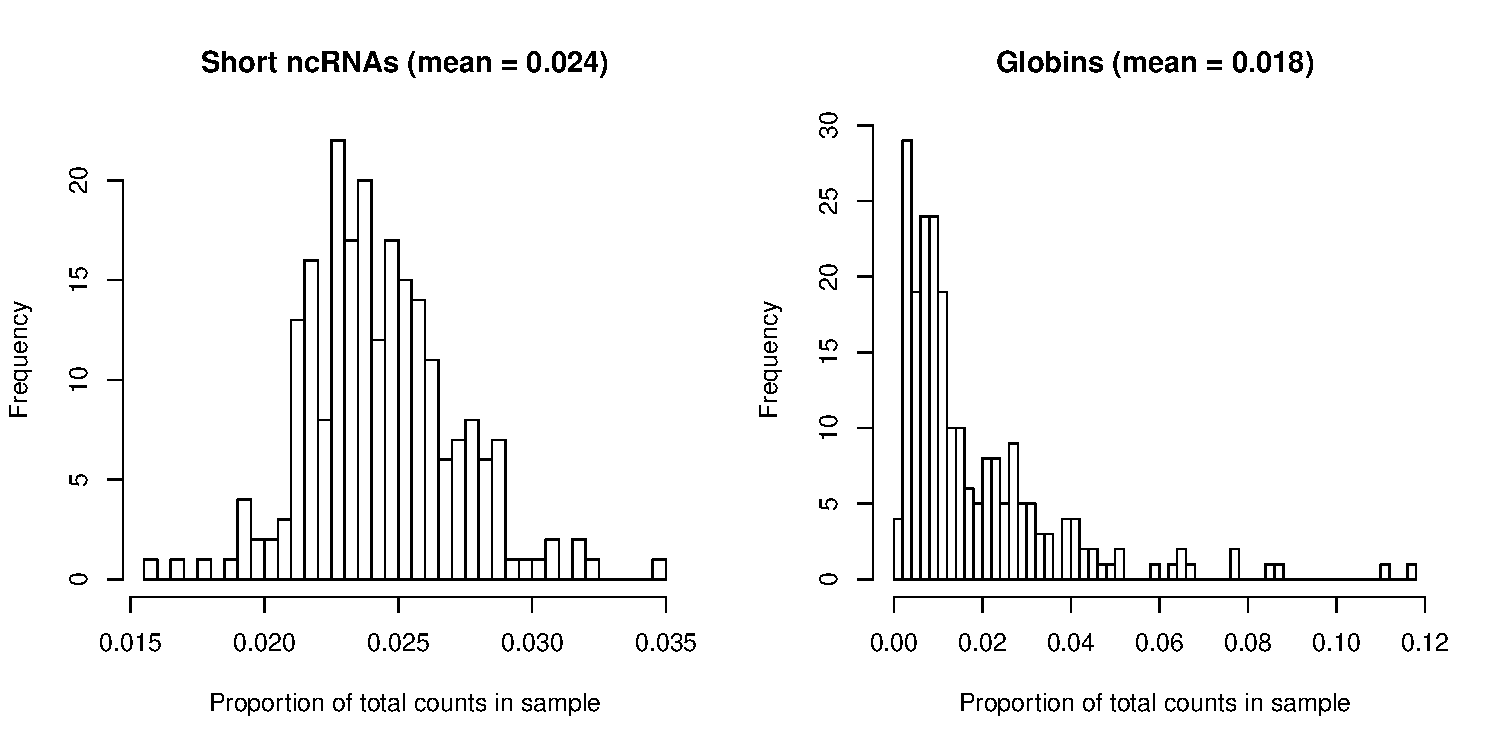
\includegraphics[width=1.0\textwidth, page=1]{./mainmatter/figures/chapter_02/rnaseq_data_setup.per_sample.short_ncRNA_globin_levels_hist.pdf}
    \caption{ncRNA and globin levels.}
\end{figure}

\begin{figure}
    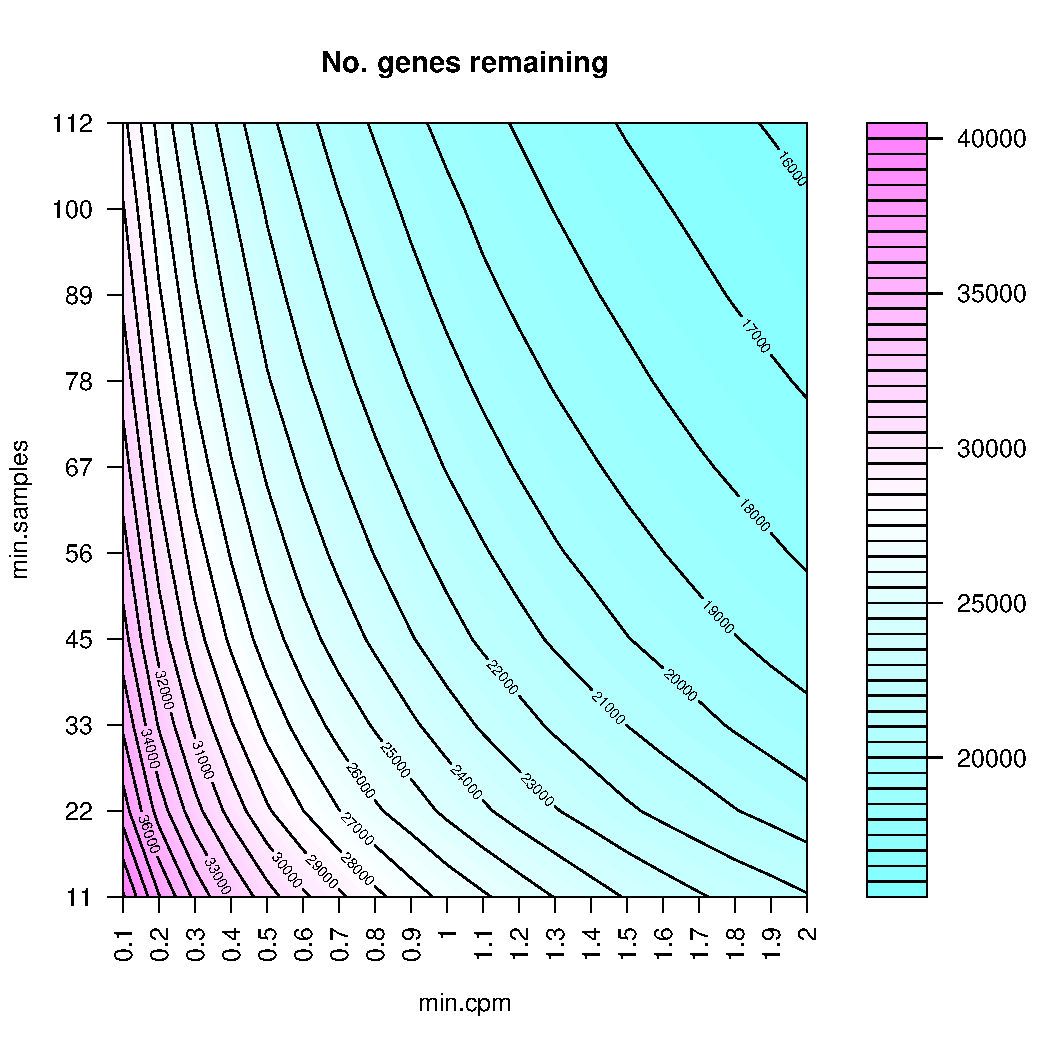
\includegraphics[width=1.0\textwidth]{./mainmatter/figures/chapter_02/rnaseq_data_setup.filtering_thresh_contour.pdf}
    \caption{Number of features retained at different thresholds.}
\end{figure}

\begin{figure}
    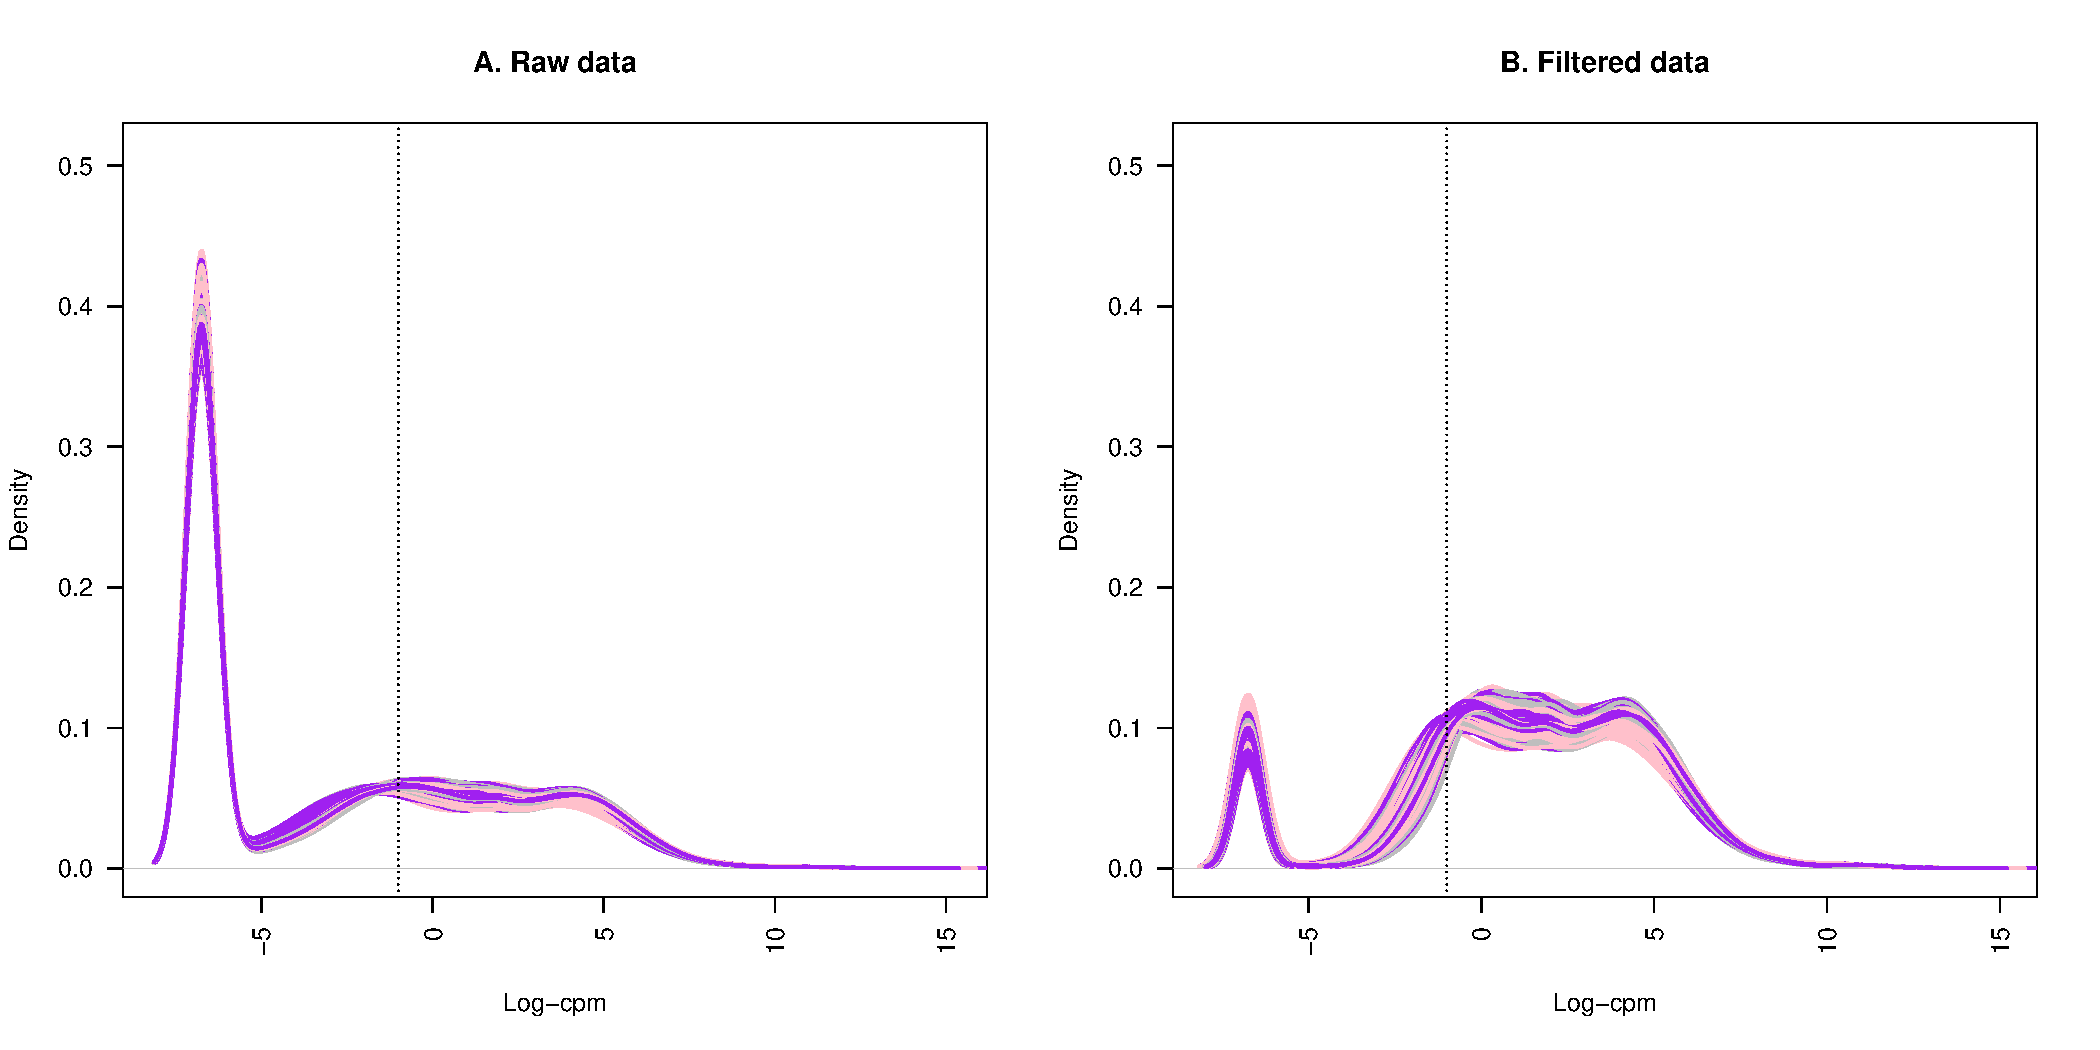
\includegraphics[width=1.0\textwidth]{./mainmatter/figures/chapter_02/rnaseq_data_setup.sample_cpm_density_filtered.pdf}
    \caption{Choice of cpm filtering threshold.}
\end{figure}

\subsection{Array data preprocessing}

\begin{outline}

% 6.	Pre-process microarray expression data
% 6.1.	Annotate Entrez and ENS ids using hgug4112a.db
% 6.1.1.	The chip is single-channel “Agilent-014850 Whole Human Genome Microarray 4x44K G4112F”
% 6.1.2.	Apparently fine to use 4112A db for 4112F https://support.bioconductor.org/p/73193/
% 6.2.	Redefine responder phenotype to be consistent with RNA-seq and Sobolev paper (>= 4-fold in HAI or MN)
% 6.3.	Background correction: limma::backgroundCorrect(x, method="normexp")
% 6.3.1.	Background comes from non-specific binding
% 6.3.2.	Pipeline from the Agi4x44PreProcess Bioconductor package (deprecated)
% 6.3.3.	Notes on Edwards: https://academic.oup.com/bioinformatics/article/23/20/2700/230165#2633725
% 6.3.3.1.	“adjusts the foreground intensities by subtracting the background when the difference between the foreground and background is larger than a small threshold value. When the difference is less than the threshold, subtraction is replaced by a smooth monotonic function.“
% 6.3.3.2.	May be preferred over normexp in our case due to “Question: Compressed boxplots after 'normexp+offset' background correction of Agilent one color microarrays in LIMMA“ https://support.bioconductor.org/p/46485/
% 6.3.3.3.	Example of Edwards used over normexp for Agilent arrays: “Modified least-variant set normalization for miRNA microarray” https://www.ncbi.nlm.nih.gov/pmc/articles/PMC2995391/
% 6.3.3.4.
% 6.3.4.	Notes on normexp:
% 6.3.4.1.	This function is designed to produce positive corrected intensities.
% 6.3.4.1.1.	“If the "normexp" method is selected, then a convolution of normal and exponential distributions is fitted to the foreground intensities using the background intensities as a covariate, and the expected signal given the observed foreground becomes the corrected intensity.”
% 6.3.4.1.2.	https://www.ncbi.nlm.nih.gov/pmc/articles/PMC2648902/ “A method normexp was introduced which models the observed intensities as the sum of exponentially distributed signals and normally distributed background values”
% 6.3.4.2.	[…] an offset value (normally 50) is used. This offset adds a constant to the intensities before log-transforming, so that the log ratios are shrunk towards zero at the lower intensities.
% 6.3.4.3.	The optimal choice for the offset is the one which makes the variability of the log-ratios as constant as possible across the range of intensity values (Smyth, G. in BioC mailing List, https://stat.ethz.ch/pipermail/bioconductor/2006-April/012554.html ).
% 6.3.5.	Choice of offset: https://academic.oup.com/nar/article/38/22/e204/1049223#93002104
% 6.3.5.1.	Adding an offset to the intensities before log transformation not only was found to lower the variance (improve precision) but also to compress the fold-change range and increase bias. In other words, offsets decrease noise but increase bias.
% 6.3.5.2.	The normexp by control (neqc) algorithm […] For routine practical use, we recommend modest offsets for Illumina data in the range of 10–50, which minimize the bias while still delivering a benefit in terms of FDR. Offsets of 16–50 have been used in a number of biological studies (10,13,16). These results remain essentially unchanged whether or not control probes are used […]  The default offset is 16, which seems generally to give good results on recent versions of human and mouse Illumina arrays.
% No need for normalizeWithinArrays in 2 color.
% 6.4.	Between-sample normalization: Limma::normalizeBetweenArrays(y, method="quantile")
% Why quantile normalise arrays? "A comparison of normalization methods for high density oligonucleotide array data based on variance and bias"
% 6.4.1.	Note that we omit any normalize within arrays procedures, as this is a single-channel array
% 6.4.2.	Normalization is the attempt to compensate for systematic technical differences between chips
% 6.4.3.	Uses https://www.rdocumentation.org/packages/limma/versions/3.28.14/topics/normalizeQuantiles
% 6.4.3.1.	“Each quantile of each column is set to the mean of that quantile across arrays. The intention is to make all the normalized columns have the same empirical distribution. This will be exactly true if there are no missing values and no ties within the columns: the normalized columns are then simply permutations of one another.”
% 6.4.4.	Also see this “StatQuest: Quantile Normalization” https://www.youtube.com/watch?v=ecjN6Xpv6SE
% 6.4.5.	This also does a log2 transform, so final units are normalized log2 intensity
% 6.5.	Summarise probes (into loci): WGCNA::collapseRows(rowGroup=Ensembl ID, method="MaxMean", connectivityBasedCollapsing=FALSE)
% 6.5.1.	https://www.ncbi.nlm.nih.gov/pmc/articles/PMC3166942/
% 6.5.1.1.	“For example, we find that in most microarray experiments performed on brain tissue it is best to choose the probe with the maximum mean expression per gene, whereas when choosing a single gene to represent a co-expression module, the optimal collapsing method depends on the goal of the analysis.”
% 6.5.1.2.	“In the case of collapsing probes to their respective gene symbols, for example, we find that the 1.max strategy (implemented by setting method = "MaxMean" and connectivityBasedCollapsing = FALSE) produces the most robust results.”
% 6.5.1.3.	i.e. choose the probe with the highest mean of expression over the samples

Batch effect correction (see batch effects Zotero tag)
% Chen, C., Grennan, K., Badner, J., Zhang, D., Gershon, E., Jin, L., & Liu, C. (2011). Removing Batch Effects in Analysis of Expression Microarray Data: An Evaluation of Six Batch Adjustment Methods. PLoS ONE, 6(2), e17238. https://doi.org/10.1371/journal.pone.0017238
Combat is best here.
% Espín-Pérez, A., Portier, C., Chadeau-Hyam, M., van Veldhoven, K., Kleinjans, J. C. S., & de Kok, T. M. C. M. (2018). Comparison of statistical methods and the use of quality control samples for batch effect correction in human transcriptome data. PLOS ONE, 13(8), e0202947. https://doi.org/10.1371/journal.pone.0202947
LM, LMM, Combat were comparable.
% Liu, Q., & Markatou, M. (2016). Evaluation of Methods in Removing Batch Effects on RNA-seq Data. Infectious Diseases and Translational Medicine, 2(1), 3–9. https://doi.org/10.11979/idtm.201601002
In some cases, Combat overcorrects.
% Nygaard, V., Rødland, E. A., & Hovig, E. (2015). Methods that remove batch effects while retaining group differences may lead to exaggerated confidence in downstream analyses. Biostatistics, (January), kxv027. https://doi.org/10.1093/biostatistics/kxv027
Main issue is unbalanced design, which affects even 2-way anova. Rather than 2-step, Safest is to use a covariate, which seems to at least create appropriate conficence intervals (1e).

\begin{figure}
\includegraphics[width=1.0\textwidth]{example-image}
\caption{TABLE: Balance of timepoints and R/NR in the two array batches.}
\end{figure}

\begin{figure}
    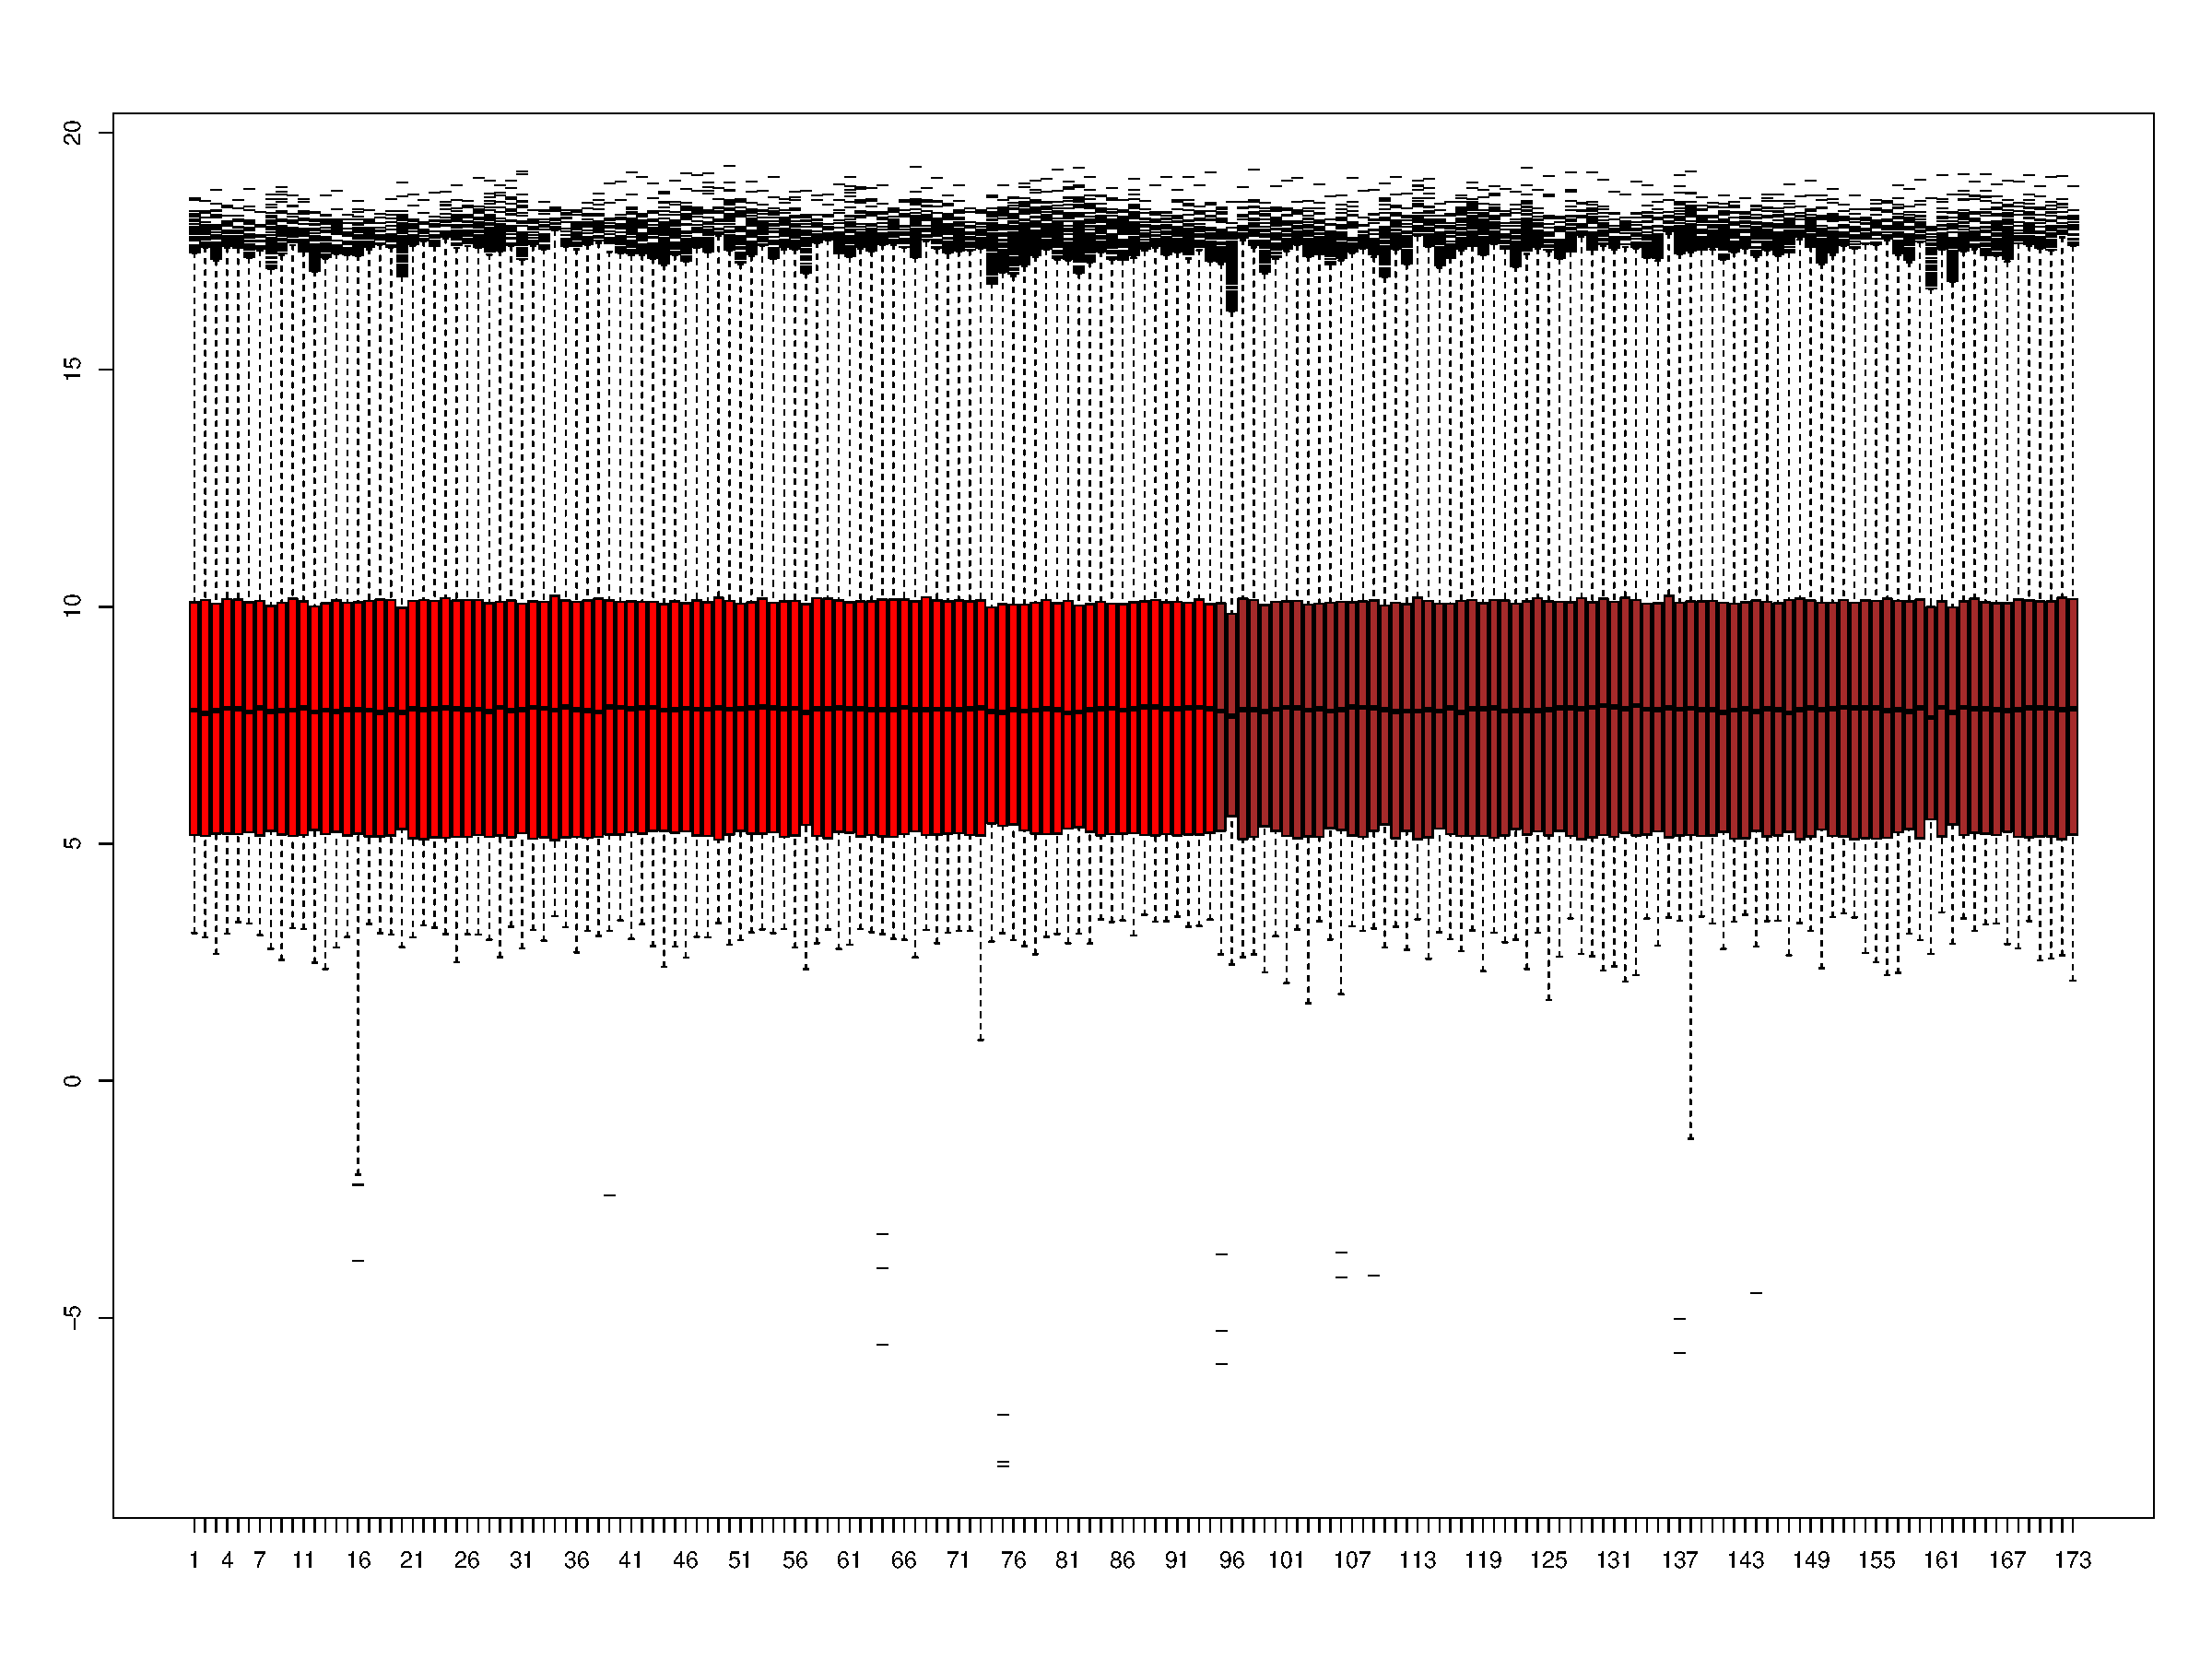
\includegraphics[width=1.0\textwidth]{./mainmatter/figures/chapter_02/array_data_setup.array_intensity_boxplots.MaxMean.combat.pdf}
    \caption{Array intensity estimates after normalisation and batch effect correction.}
\end{figure}

\end{outline}

\subsection{Computing baseline-adjusted measure of antibody response: \glsfmtshort{TRI}}

\begin{outline}
\1 Pre-process phenotypes
    \2 Compute responder status (>= 4-fold in HAI or MN)
    \2 Compute TRI (based on Bucasas 2009)
        \3 “We related the change in titer between pre- and postvaccination measurements (response variable) to the prevaccination titer (explanatory variable) using a simple linear model”
        \3 “We next determined the residuals from the above linear regressions and used them as the input values for the individual response scores.”
        \3 “we standardized the residuals by dividing by the residual standard deviation for each component”
            \4 Based on their axis ranges, it appears they are plotting log2(post)-log2(pre)), equivalently log2(post/pre), a.k.a. log2 fold-change; against log2(pre)
            \4 Note that log2(post-pre) does not make sense mathematically, as post-pre may well be negative
            \4 The negative relationship indicates lower initial titres are more amenable to high fold-change increases, which is exactly what TRI is designed to correct for
\1 We computed TRI for the HIRD dataset (Fig. \ref{fig:tri_vs_fc})
\1 Relationship between TRI and the clinical responder definition used by Sobolev et al. (Fig. \ref{fig:tri_vs_responder}).
\end{outline}

\begin{figure}
    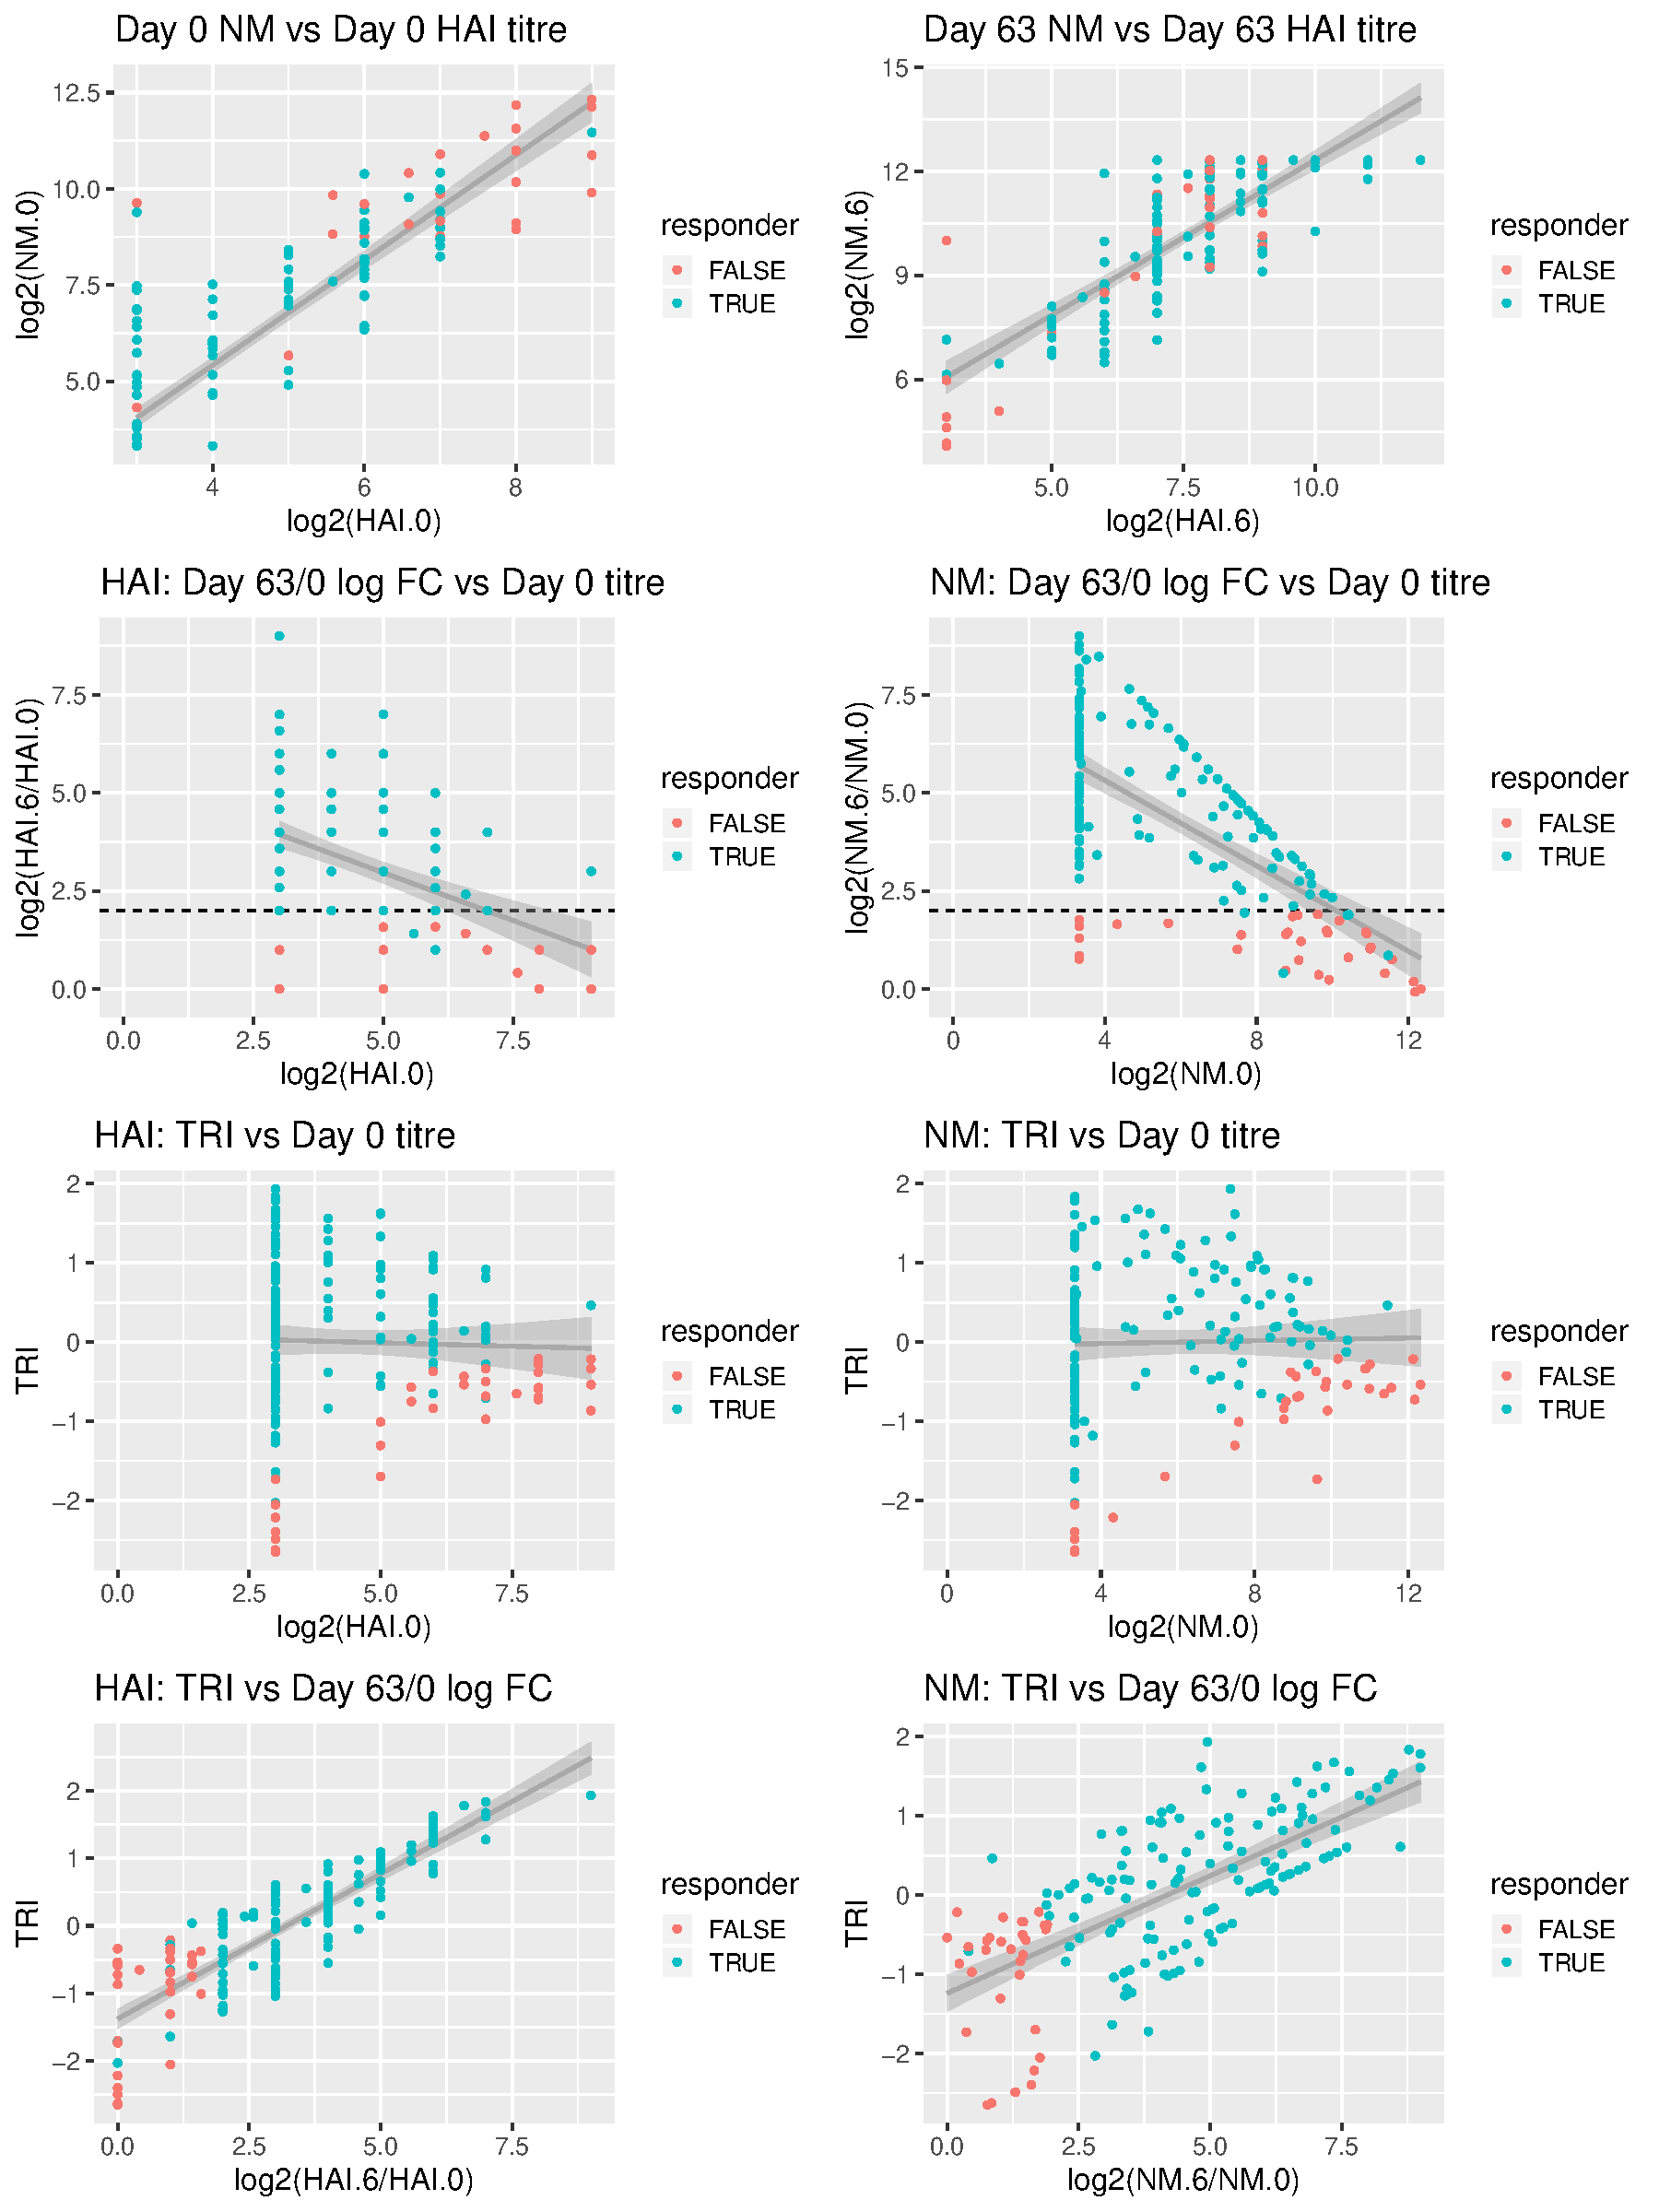
\includegraphics[width=1.0\textwidth]{./mainmatter/figures/chapter_02/phenotype_data_setup.tri_comparison.pdf}
    \caption{How TRI corrects fold changes for baseline titre.}
    \label{fig:tri_vs_fc}
\end{figure} 

\begin{figure}
    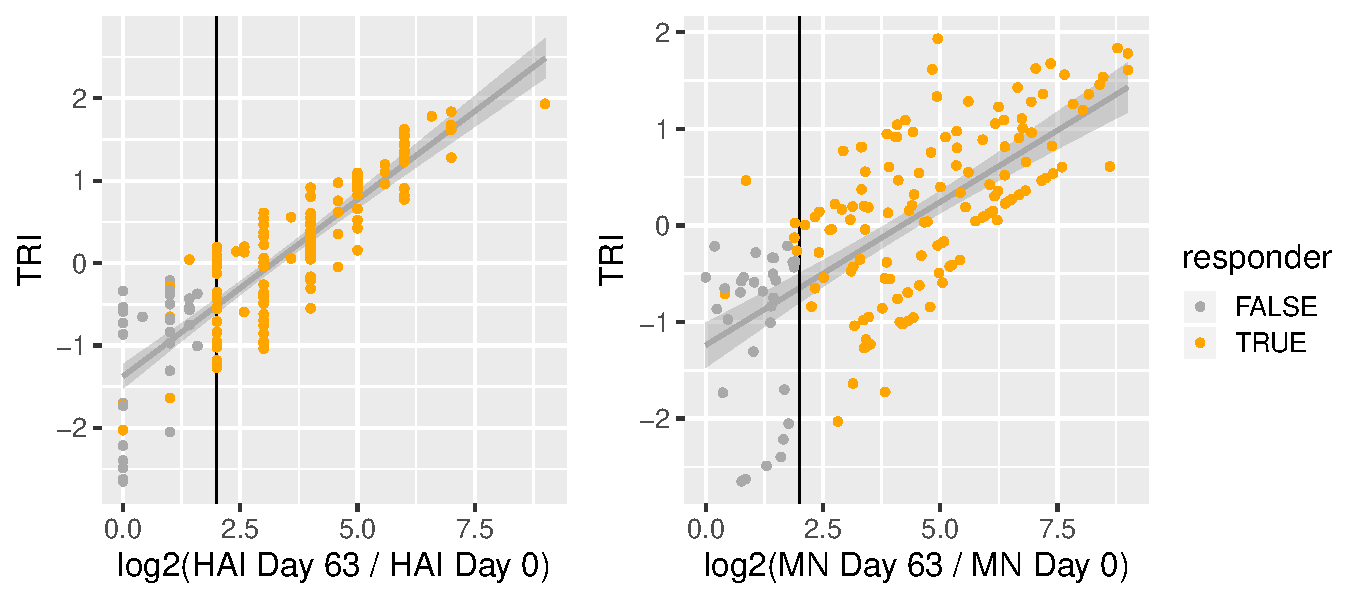
\includegraphics[width=1.0\textwidth]{./mainmatter/figures/chapter_02/phenotype_data_setup.tri_comparison_ASHG.pdf}
    \caption{TRI correlates with the standard responder definition (colored, 4-fold increase in either assay). An individual's TRI is the mean of their Z-transformed residuals from regressions of day 63 vs. day 0 fold-change against day 0 titre, over the two assays.}
    \label{fig:tri_vs_responder}
\end{figure}

\subsection{\Glsfmtfull{DGE}}

\begin{figure}
    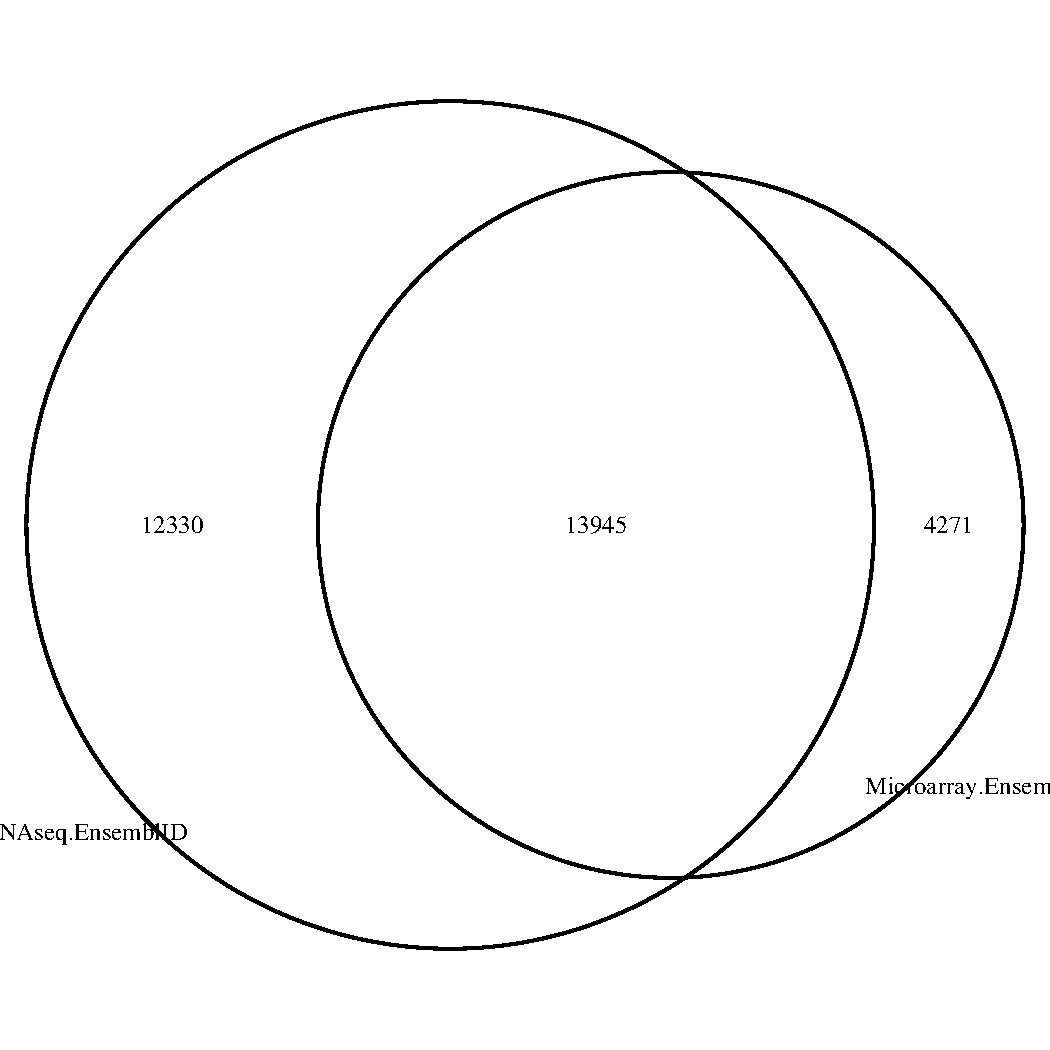
\includegraphics[width=1.0\textwidth]{./mainmatter/figures/chapter_02/array_data_setup.rnaseqFeatureOverlap.Ensembl.postFiltering.pdf}
    \caption{Feature overlap between array and RNAseq data post-filtering.}
\end{figure}

Why limma over edgeR/DESeq2?
Comparable at sufficient sample sizes, and faster.

Why combine -7 and 0?
See Sobolev: (a) Observed values of multivariate statistic t (m.v.t.) quantifying global PBMC gene-expression dissimilarity in comparison of two study days (red dots) to values expected when days are randomly assigned between groups.

% 7.	Differential expression (limma)
% 7.2.	Create contrasts
% 7.2.1.	Combat or not? See: https://support.bioconductor.org/p/72815/
% 7.3.	Estimate within-block correlation (duplicateCorrelation), using patients as blocks
% 7.4.	Array data only: Compute sample quality weights for each array (arrayWeightsSimple(v, design=mod1))
% 7.5.	RNA-seq data only: Correct for mean-variance trend (voom)
% 7.5.1.	http://web.mit.edu/~r/current/arch/i386_linux26/lib/R/library/limma/html/voom.html
% 7.5.1.1.	“voom is an acronym for mean-variance modelling at the observational level. The key concern is to estimate the mean-variance relationship in the data, then use this to compute appropriate weights for each observation. Count data almost show non-trivial mean-variance relationships. Raw counts show increasing variance with increasing count size, while log-counts typically show a decreasing mean-variance trend. This function estimates the mean-variance trend for log-counts, then assigns a weight to each observation based on its predicted variance. The weights are then used in the linear modelling process to adjust for heteroscedasticity.”
% 7.5.1.2.	“voom performs the following specific calculations. First, the counts are converted to logCPM values, adding 0.5 to all the counts to avoid taking the logarithm of zero. The matrix of logCPM values is then optionally normalized. The lmFit function is used to fit row-wise linear models. The lowess function is then used to fit a trend to the square-root-standard-deviations as a function of average logCPM. The trend line is then used to predict the variance of each logCPM value as a function of its fitted value, and the inverse variances become the estimated precision weights.”
% 7.6.	(lmFit)
% 7.7.	(contrasts.fit)
% 7.8.	(eBayes/treat)
% 7.8.1.1.1.	https://rdrr.io/bioc/limma/man/ebayes.html
% 7.8.1.1.1.1.	When lfc=0, treat is identical to eBayes, except that F-statistics and B-statistics are not computed.
% 7.8.1.1.2.	https://academic.oup.com/bioinformatics/article/25/6/765/251641 The TREAT fold-change threshold should be set to a low value below which no fold-change is likely to be of genuine interest. Researchers should be mindful that genes will need to exceed this threshold by some way, depending on the data, before being declared statistically significant. Our experience suggests a minimal value, such as a 10% fold-change, corresponding to τ=log2(1.1)=0.13 on the log2-scale. It would be better to interpret the threshold as ‘the fold-change below which we are definitely not interested in the gene’ rather than ‘the fold-change above which we are interested in the gene’.
% 7.9.	(decideTests)

Equation for linear models used in limma.

\subsection{\glsfmtshort{DGE} meta-analysis}

Should we meta-analyse?
% https://journals.plos.org/plosone/article?id=10.1371/journal.pone.0059202
"In conclusion, we found that underpowered studies play a very substantial role in meta-analyses reported by Cochrane reviews, since the majority of meta-analyses include no adequately powered studies. In meta-analyses including two or more adequately powered studies, the remaining underpowered studies often contributed little information to the combined results, and could be left out if a rapid review of the evidence is required."

\subsubsection{Cross-platform meta-analysis methods}

\begin{outline}

\1 Whilst there is a slew of literature on meta-analysis of rnaseq and array (e.g. metaMA), combining platforms is fraught with difficulties.
    \2 different tech -> diff statistical models

\1 Expected heterogeneity:
    \2 Platform effect (ratio compression, differences in preprocessing to genes). 
    \2 Different sets of samples (more extreme in array)

\1 Examples of past meta:
    \2 sva: https://www.ncbi.nlm.nih.gov/pmc/articles/PMC3617154/

    \2 MetaVolcano: vote counting, REM (note small k)

    \2 CorMotif first applies limma (Smyth, 2004) to each study separately.
        \3 CorMotif for microarray data since it was motivated by the microarray analysis in the SHH study. However, the idea behind CorMotif is general, and it should be straightforward to develop a similar framework for RNA-seq data.

    \2 CBM (“Cross-platform Bayesian Model”), see CBM paper for discussion of difficulties of combinding platform
        \3 cannot acually use CBM, as it operates on expressions, with a binary case vs control, so no covariates
        \3 same limitation for cormotif, although it takes any number of groups

    \2 Rankprod (focus on case/control design)
    \2 Mayday seasight

\1 Classic models: Two schools of thought for frequentist meta-analysis: 
    \2 fixed-effect
    % Higgins, J. P. T., Thompson, S. G., & Spiegelhalter, D. J. (2009). A re-evaluation of random-effects meta-analysis. Journal of the Royal Statistical Society: Series A (Statistics in Society), 172(1), 137–159. https://doi.org/10.1111/j.1467-985X.2008.00552.x
    \2 or in the presence of het, random-effects.
        % https://academic.oup.com/nar/article/45/17/9860/4084660#106485896
        \3 e.g. random effects model of approx 24 datasets

    \2 We have het, so def use random effects.

% Veroniki, A. A., Jackson, D., Viechtbauer, W., Bender, R., Bowden, J., Knapp, G., … Salanti, G. (2016). Methods to estimate the between-study variance and its uncertainty in meta-analysis. Research Synthesis Methods, 7(1), 55–79. https://doi.org/10.1002/jrsm.1164
\1 How to estimate het?
    % Gonnermann, A., Framke, T., Großhennig, A., & Koch, A. (2015). Nosolution yet for combining two independent studies in the presence of heterogeneity: COMMENTARY. Statistics in Medicine, 34(16), 2476–2480. https://doi.org/10.1002/sim.6473
    % Friede, T., Röver, C., Wandel, S., & Neuenschwander, B. (2017). Meta-analysis of few small studies in orphan diseases: Meta-Analysis of Few Small Studies. Research Synthesis Methods, 8(1), 79–91. https://doi.org/10.1002/jrsm.1217
    % Friede, T., Röver, C., Wandel, S., & Neuenschwander, B. (2017). Meta-analysis of two studies in the presence of heterogeneity with applications in rare diseases: Meta-analysis of two studies in the presence of heterogeneity. Biometrical Journal, 59(4), 658–671. https://doi.org/10.1002/bimj.201500236
    % Seide, S. E., Röver, C., & Friede, T. (2019). Likelihood-based random-effects meta-analysis with few studies: Empirical and simulation studies. BMC Medical Research Methodology, 19(1). https://doi.org/10.1186/s12874-018-0618-3
    \2 Many methods and estimators.

    \2 The problem: we only have k=2, and MLE estimates of tau are not very good with k=2.
        % Sweeny "Methods to increase reproducibility in differential"
        \3 Sweeny tests the effect of varying k.
        \3 Highly imprecise, and often boundary estimate problems, and we know 0 het is inappropriate.
        % Chung, Y., Rabe-Hesketh, S., Dorie, V., Gelman, A., & Liu, J. (2013). A Nondegenerate Penalized Likelihood Estimator for Variance Parameters in Multilevel Models. Psychometrika, 78(4), 685–709. https://doi.org/10.1007/s11336-013-9328-2

% Friede, T., Röver, C., Wandel, S., & Neuenschwander, B. (2017). Meta-analysis of few small studies in orphan diseases: Meta-Analysis of Few Small Studies. Research Synthesis Methods, 8(1), 79–91. https://doi.org/10.1002/jrsm.1217
% Friede, T., Röver, C., Wandel, S., & Neuenschwander, B. (2017). Meta-analysis of two studies in the presence of heterogeneity with applications in rare diseases: Meta-analysis of two studies in the presence of heterogeneity. Biometrical Journal, 59(4), 658–671. https://doi.org/10.1002/bimj.201500236
% Seide, S. E., Röver, C., & Friede, T. (2019). Likelihood-based random-effects meta-analysis with few studies: Empirical and simulation studies. BMC Medical Research Methodology, 19(1). https://doi.org/10.1186/s12874-018-0618-3
\1 Bayesian random-effects meta is attractive, but what priors should we use?

\end{outline}

\subsubsection{Prior for between-studies heterogeneity}

\begin{outline}

Prior for tau.

% Gelman (2006)
\1 A general rec is: Use distribution in the half-t family e.g. Cauchy (df=1) when the number of groups is small and in other settings where a weakly-informative prior is desired.
    \2 In their 3-schools examples, choose a value of scale just higher than expected, this is to weakly constrain the posterior, and not to actually represent prior knowledge.
    \2 Warn against inverse-gamma(e, e), as it can influence the posterior mean.

% Friede, T., Röver, C., Wandel, S., & Neuenschwander, B. (2017). Meta-analysis of few small studies in orphan diseases: Meta-Analysis of Few Small Studies. Research Synthesis Methods, 8(1), 79–91. https://doi.org/10.1002/jrsm.1217
% Friede, T., Röver, C., Wandel, S., & Neuenschwander, B. (2017). Meta-analysis of two studies in the presence of heterogeneity with applications in rare diseases: Meta-analysis of two studies in the presence of heterogeneity. Biometrical Journal, 59(4), 658–671. https://doi.org/10.1002/bimj.201500236
% Seide, S. E., Röver, C., & Friede, T. (2019). Likelihood-based random-effects meta-analysis with few studies: Empirical and simulation studies. BMC Medical Research Methodology, 19(1). https://doi.org/10.1186/s12874-018-0618-3
\1 But weak priors are not recommended, as k is small, so there is little information in the data.
% https://github.com/stan-dev/stan/wiki/Prior-Choice-Recommendations
% The Gelman (2006) half-cauchy may be too weak for small k.

\1 We can get empirical distribution of many genes.
    % see this for a justification of why REML over ML
    % Veroniki, A. A., Jackson, D., Viechtbauer, W., Bender, R., Bowden, J., Knapp, G., … Salanti, G. (2016). Methods to estimate the between-study variance and its uncertainty in meta-analysis. Research Synthesis Methods, 7(1), 55–79. https://doi.org/10.1002/jrsm.1164
    \2 fit a default reml model, exclude 0 ests.
    % By default, the starting value is set equal to the value of the Hedges (HE) estimator and the algorithm terminates when the change in the estimated value of  2 is smaller than 105 from one iteration to the next.
\1 Advantage of getting the correct parameter scale for our data.
\1 So use Empirical Bayes:
    \2 aside: empirical bayes is popular for high dim data e.g. edgeR, DESeq2, limma-voom, combat (method of moments)

\1 Papers that fit empirical datasets for tau2: Most of these are inverse-gamma/log-t family
    % Higgins, J. P. T., & Whitehead, A. (1996). Borrowing strength from external trials in a meta-analysis. Statistics in Medicine, 15(24), 2733–2749. https://doi.org/10.1002/(SICI)1097-0258(19961230)15:24<2733::AID-SIM562>3.0.CO;2-0
    \2 Fit inverse gamma distribution on method of moments estimates from 18 gastroenterology trials with similar endpoints.
    % Pullenayegum, E. M. (2011). An informed reference prior for between-study heterogeneity in meta-analyses of binary outcomes: Prior for between-study heterogeneity. Statistics in Medicine, 30(26), 3082–3094. https://doi.org/10.1002/sim.4326
    \2 This paper has described the distribution of the between-study variance amongst Cochrane reviews published between 2008 and 2009, and investigating a binary outcome. A log-normal distribution incorporating the association between the between-study variance and the pooled effect size gave the best fit.
    % Turner, R. M., Davey, J., Clarke, M. J., Thompson, S. G., & Higgins, J. P. (2012). Predicting the extent of heterogeneity in meta-analysis, using empirical data from the Cochrane Database of Systematic Reviews. International Journal of Epidemiology, 41(3), 818–827. https://doi.org/10.1093/ije/dys041
    \2 Predictive distributions are presented for nine different settings, defined by type of outcome and type of intervention comparison. For example, for a planned meta-analysis comparing a pharmacological intervention against placebo or control with a subjectively measured outcome, the predictive distribution for heterogeneity is a log-normal (2.13, 1.582) distribution, which has a median value of 0.12.
    % Rhodes, K. M., Turner, R. M., & Higgins, J. P. T. (2015). Predictive distributions were developed for the extent of heterogeneity in meta-analyses of continuous outcome data. Journal of Clinical Epidemiology, 68(1), 52–60. https://doi.org/10.1016/j.jclinepi.2014.08.012
    \2 Model selection based on the deviance information criterion (DIC) [8] led to the choice of the log-t model for t2. (5df)
    % Turner, R. M., Jackson, D., Wei, Y., Thompson, S. G., & Higgins, J. P. T. (2015). Predictive distributions for between-study heterogeneity and simple methods for their application in Bayesian meta-analysis: R. M. TURNER ET AL. Statistics in Medicine, 34(6), 984–998. https://doi.org/10.1002/sim.6381
    \2 The priors are derived as log-normal distributions for the between-study variance, applicable to meta-analyses of binary outcomes on the log odds-ratio scale.

% Chung, Y., Rabe-Hesketh, S., Dorie, V., Gelman, A., & Liu, J. (2013). A Nondegenerate Penalized Likelihood Estimator for Variance Parameters in Multilevel Models. Psychometrika, 78(4), 685–709. https://doi.org/10.1007/s11336-013-9328-2
\1 We choose gamma: as Density at tau=0 is 0, but increases linearly from 0, so values close to 0 are still permitted if the data suggests it.
    \2 For lognormal/inverse gamma, they have a derivative of 0 at tau=0, so they rule out small tau no matter what the data suggest.
    \2 For The exponential and half-Cauchy families, for example, do not decline to zero at the boundary, so they do not rule out posterior mode estimates of zero.

% Maximum-likelihood Fitting of Univariate Distributions
% https://stat.ethz.ch/R-manual/R-devel/library/MASS/html/fitdistr.html
% For the Normal, log-Normal, geometric, exponential and Poisson distributions the closed-form MLEs (and exact standard errors) are used, and start should not be supplied.
% For all other distributions, direct optimization of the log-likelihood is performed using optim.
\end{outline}

\subsubsection{Prior for \glsfmtshort{DGE} effect size}

\begin{outline}

Prior for logFC

\1 Not as much discussion in the lit:
% Gelman (2006)
\1 There is Typically enough data to estimate this to use a non informative prior.
% Friede, T., Röver, C., Wandel, S., & Neuenschwander, B. (2017). Meta-analysis of few small studies in orphan diseases: Meta-Analysis of Few Small Studies. Research Synthesis Methods, 8(1), 79–91. https://doi.org/10.1002/jrsm.1217
% Friede, T., Röver, C., Wandel, S., & Neuenschwander, B. (2017). Meta-analysis of two studies in the presence of heterogeneity with applications in rare diseases: Meta-analysis of two studies in the presence of heterogeneity. Biometrical Journal, 59(4), 658–671. https://doi.org/10.1002/bimj.201500236
\1 Even Friede uses noninformative flat.

\1 Two choices in bayesmeta are uniform and normal.
    \2 We know Mean is 0: most genes are not DE, so flat prior makes no sense

% Also: general principles point towards weaker priors, but not uniform????
% https://github.com/stan-dev/stan/wiki/Prior-Choice-Recommendations
% For example, it is common to expect realistic effect sizes to be of order of magnitude 0.1 on a standardized scale (for example, an educational innovation that might improve test scores by 0.1 standard deviations). In that case, a prior of N(0,1) could be considered very strong, in that it puts most of its mass on parameter values that are unrealistically large in absolute value. When we say this prior is "weakly informative," what we mean is that, if there's a reasonably large amount of data, the likelihood will dominate, and the prior will not be important. If the data are weak, though, this "weakly informative prior" will strongly influence the posterior inference. The phrase "weakly informative" is implicitly in comparison to a default flat prior.
% Weakly informative prior should contain enough information to regularize: the idea is that the prior rules out unreasonable parameter values but is not so strong as to rule out values that might make sense
% Weakly informative rather than fully informative: the idea is that the loss in precision by making the prior a bit too weak (compared to the true population distribution of parameters or the current expert state of knowledge) is less serious than the gain in robustness by including parts of parameter space that might be relevant. It's been hard for us to formalize this idea.
% One principle: write down what you think the prior should be, then spread it out. The idea is that the cost of setting the prior too narrow is more severe than the cost of setting it too wide. I've been having trouble formalizing this idea.
% Don't use uniform priors, or hard constraints more generally, unless the bounds
% represent true constraints (such as scale parameters being restricted to be
% positive, or correlations restricted to being between -1 and 1).

\1 To avoid overshrinking, could consider heavy-tailed priors (e.g. cauchy) for mu rather than normal
    % Gelman, A., Jakulin, A., Pittau, M. G., & Su, Y.-S. (2008). A weakly informative default prior distribution for logistic and other regression models. The Annals of Applied Statistics, 2(4), 1360–1383. https://doi.org/10.1214/08-AOAS191
    \2 Cauchy 2.5
    % Zhu, A., Ibrahim, J. G., & Love, M. I. (2018). Heavy-tailed prior distributions for sequence count data: Removing the noise and preserving large differences. BioRxiv. https://doi.org/10.1101/303255
    \2 DEseq/apeglm: prior on logfc, cauchy with scale adapted.

\1 But this is not possible in bayesmeta, bayesmeta is normal. So weaken further to place more prior on larger values. This means less shrinkage.

\1 Also: we will shrink again with ashr, which can fit a more complicated (mixture?) distr

% https://github.com/stan-dev/stan/wiki/Prior-Choice-Recommendations
\1 So we use a very weak normal prior, scaled to each coef, as we still want some scaling based on parameter scales.
    \2 Equiv to saying 95pc chance that effect is within log2FC of 20.
    % > qnorm(0.975, 0, 10)
    % [1] 19.59964

% Two examples to demonstrate: the top 2 in RMA meta-analysis.
% (see section of code at end of 6.0\_de\_meta.R script)

\end{outline}

\subsubsection{Meta-analysis using bayesmeta}

\begin{figure}
    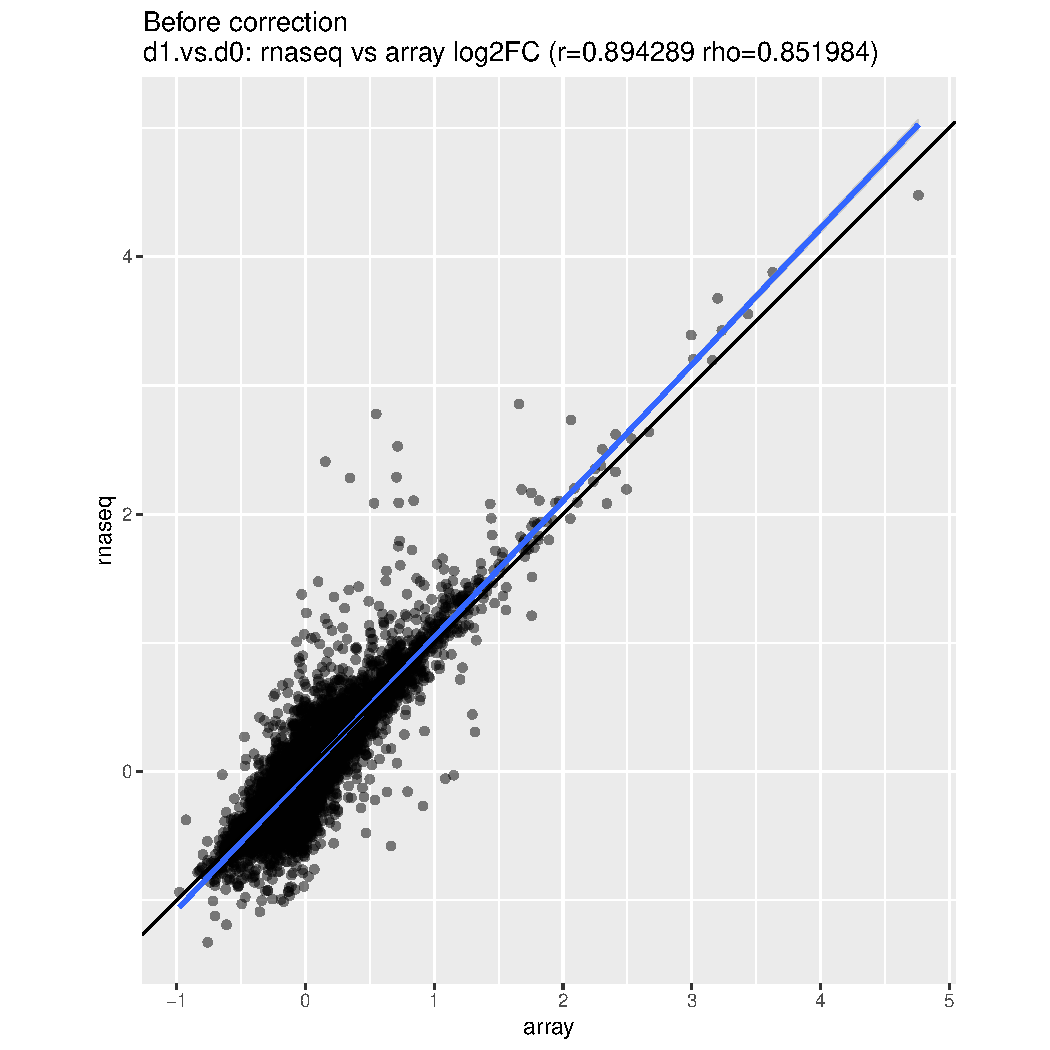
\includegraphics[width=1.0\textwidth]{./mainmatter/figures/chapter_02/meta.rnaseqVsArray.log2FC.beforeBiasCorrection.coefName_d1.vs.d0.pdf}
    \caption{Fold-change comparison between array and RNAseq for day 1 vs day 0.}
\end{figure}

\begin{figure}
    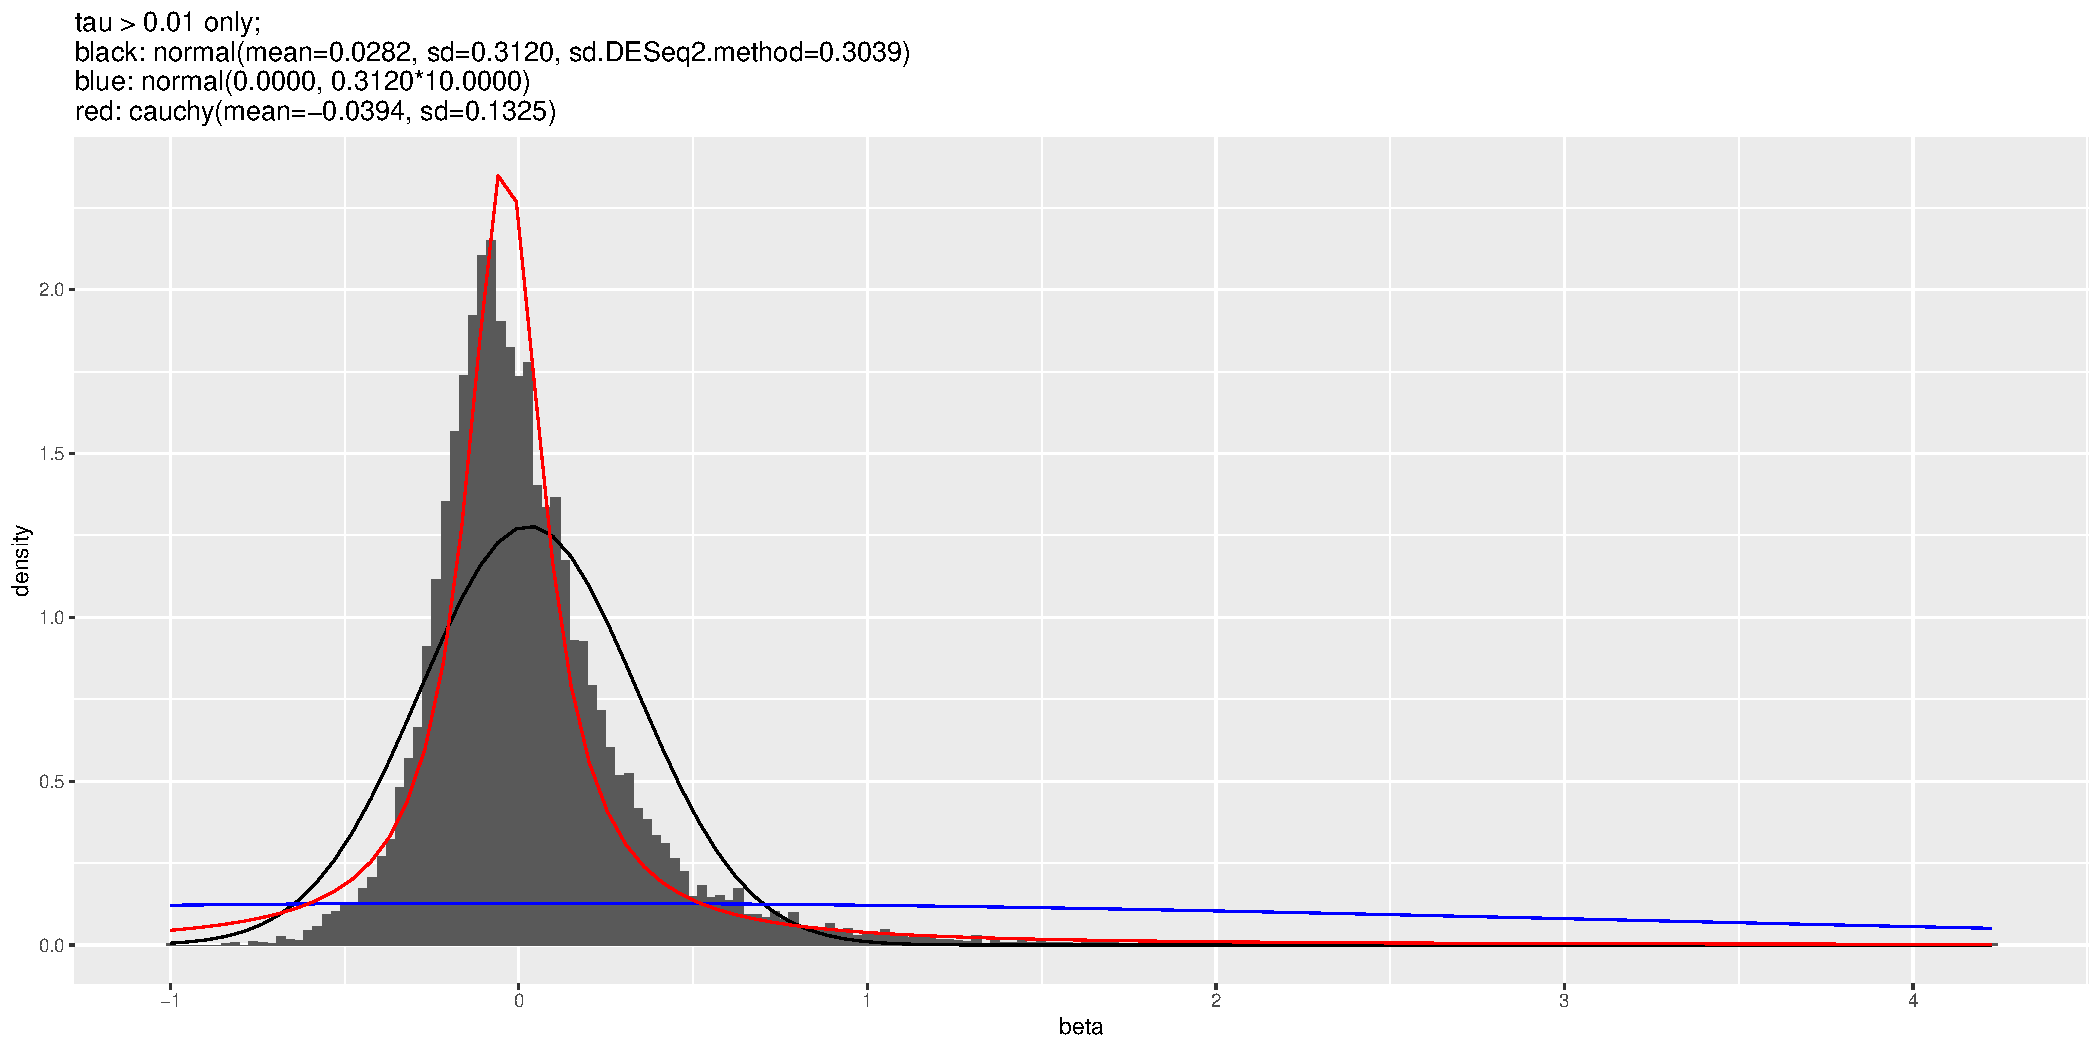
\includegraphics[width=1.0\textwidth]{./mainmatter/figures/chapter_02/meta.bayesmeta.priors.coefName_d1.vs.d0.pdf}
    \caption{Priors for day 1 vs day 0 DGE meta-analysis.}
\end{figure}

\subsection{Gene set enrichment analysis}

tmod; gprofileR; CAMERA

\section{Results}

\subsection{Innate and adaptive immune response to Pandemrix}

% TODO: check out proper way to do figure references
Overall response clusters into two distinct patterns (Fig. \ref{fig:dge_heatmap}).

Day 1 response is characterised by innate response: monocyte genes, inflammatory response, type I interferon response.
Note type I interferons are alpha/beta, not gamma.
Day 7 response is characterised by adaptive B cell response: plasma cell genes, immunoglobulins, proliferation (Table \ref{tab:tmod_dge}).

\begin{figure}
    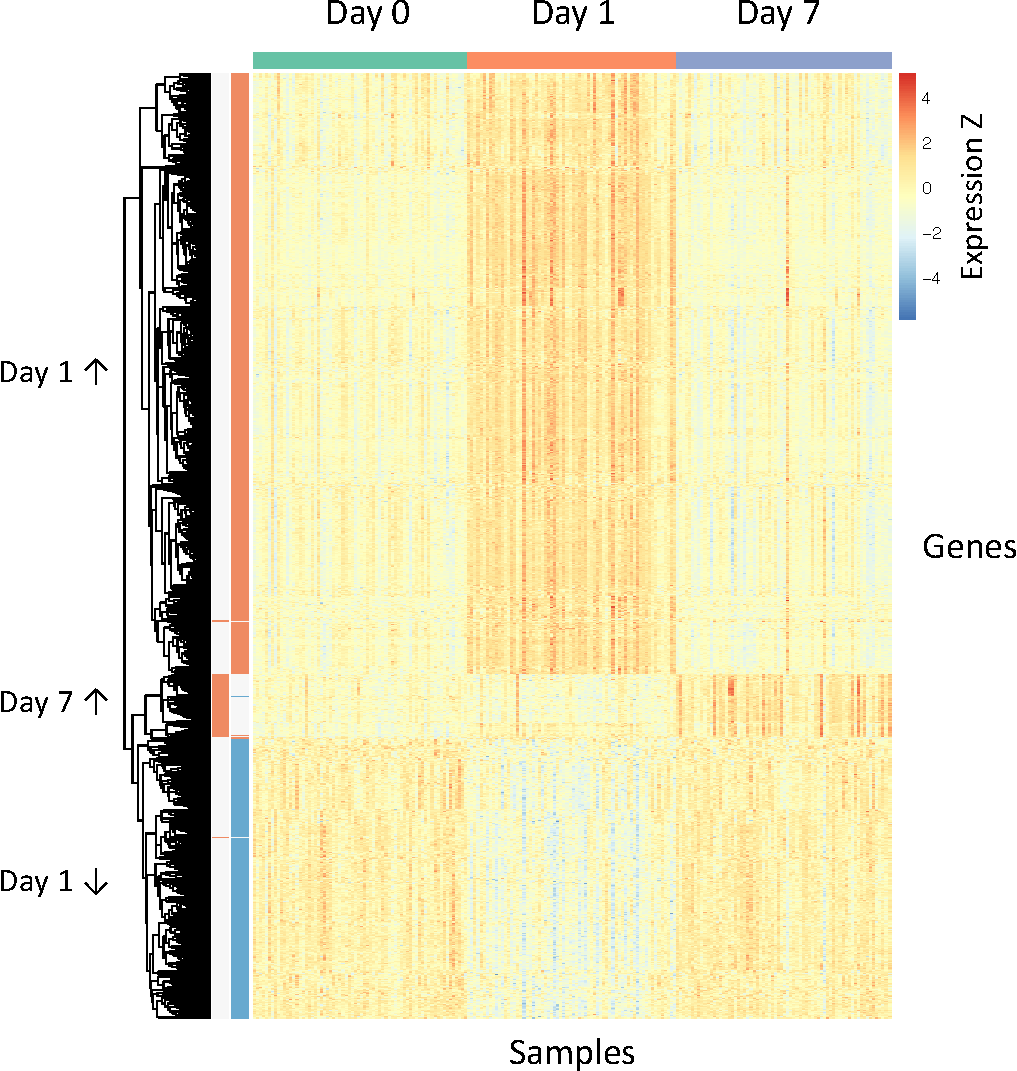
\includegraphics[width=1.0\textwidth]{./mainmatter/figures/chapter_02/graphics/plot_dge_eqtl.heatmap_dge.annotated-crop.pdf}
    \caption{Normalised gene expression for differentially expressed genes ($\text{adj. p} < 0.05$, $\left|\log_2\text{FC}\right| > 1.5$) across 208 RNA-seq samples from days 0, 1, and 7, clustered by gene.}
    \label{fig:dge_heatmap}
\end{figure}

\begin{table}
\centering
\caption{Transcriptomic modules enriched in highly up/downregulated genes in each expression cluster, based on ranking of $\log_2\text{FC}$ vs. day 0. Blank cells n.s.}
\label{tab:tmod_dge}
\sisetup{
    table-format=1.1e2,
    scientific-notation=true,
    round-mode=places,
    round-precision=1
}
\begin{adjustbox}{width=\textwidth, center}
\begin{tabular}{lSSS}  
    \toprule
        & 
        \multicolumn{3}{c}{adj. p value} \\
    \cmidrule(r){2-4}
        \multicolumn{1}{l}{Module} &
        \multicolumn{1}{c}{Day 1 $\uparrow$} &
        \multicolumn{1}{c}{Day 1 $\downarrow$} &
        \multicolumn{1}{c}{Day 7 $\uparrow$} \\
    \midrule
        cell cycle and transcription & \num{2.305733e-36} &  & \num{7.668931e-61} \\
        %
        immune activation - generic cluster & \num{1.384615e-32} & & \\
        enriched in monocytes & \num{2.852435e-90} & & \\
        TLR and inflammatory signaling & \num{1.734079e-28} & & \\
        type I interferon response & \num{8.924156e-13} & & \\
        %
        cell division stimulated CD4+ T cells & & & \num{3.478934e-18} \\
        PLK1 signaling events & & & \num{2.719531e-25} \\
        plasma cells, immunoglobulins & & & \num{5.821306e-12} \\
        %
        enriched in NK cells & & \num{4.871453e-50} & \\
        enriched in T cells & & \num{3.773967e-46} & \\
        T cell activation & & \num{8.704655e-29} & \\
    \bottomrule
\end{tabular}
\end{adjustbox}
\end{table}

\subsubsection{TODO Comparison to Sobolev et al.}

\subsection{Expression associated with antibody response}

\begin{outline}
\1 Overall, B cell module positively associated, inflammatory modules negatively associated with TRI (Table \ref{tab:tmod_tri}).
\1 TODO: split by day and look for signatures per day
\end{outline}

\begin{table}
\centering
\caption{Transcriptomic modules enriched in genes with expression positively and negatively associated with TRI. Blank cells n.s.}
\label{tab:tmod_tri}
\sisetup{
    table-format=1.1e2,
    scientific-notation=true,
    round-mode=places,
    round-precision=1
}
\begin{adjustbox}{width=\textwidth, center}
\begin{tabular}{lSS}  
    \toprule
        & 
        \multicolumn{2}{c}{adj. p value} \\
    \cmidrule(r){2-3}
        \multicolumn{1}{l}{Module} &
        \multicolumn{1}{c}{High TRI} &
        \multicolumn{1}{c}{Low TRI} \\
    \midrule
        plasma cells \& B cells, immunoglobulins & \num{0.0007953038} & \\
        % detect the presence of cytosolic DNA and, in response, trigger expression of inflammatory genes that can lead to senescence[1] or to the activation of defense mechanisms. DNA is normally found in the nucleus of the cell.
        innate activation by cytosolic DNA sensing & & \num{0.00374710} \\
        % too much inflam is detrimental?
        proinflammatory cytokines and chemokines & & \num{0.00374710} \\
        % transcription factor activator protein 1 (AP‐1) is proving to be an important regulator of nuclear gene expression in leukocytes.
        AP-1 transcription factor network & & \num{0.01418659} \\
        enriched in neutrophils & & \num{0.02281710} \\
    \bottomrule
\end{tabular}
\end{adjustbox}
\end{table}

\subsubsection{TODO Comparison to Sobolev et al.}

\subsection{TODO Identifying molecular signatures for predicting antibody response}

\begin{outline}

\1 For inference, don't dichotimise due to statistical concerns
    % Nauta JJ, Beyer WE, Osterhaus AD. On the relationship between mean antibody level, seroprotection and clinical protection from influenza. Biologicals 2009; 37:216-21; PMID:19268607; http://dx. doi.org/10.1016/j.biologicals.2009.02.002
    \2 "In clinical studies seroprotection is normally defined as a specific antibody titer or antibody titer increase (seroconversion)."
    \2 For prediction, what rules can be easily implemented in the clinic?

\1 Interpretatability: DAMIP gives rulesets composed of small sets of genes, amenable to rapid qPCR assays.

\end{outline}

\section{Discussion}

Recap of results with limitations
\begin{outline}
% "Sobolev et al. identify an early interferon and lymphoid response that can be seen 1 day after vaccination2. These signals have not been detected in other studies, but this might be explained by differences in vaccine formulation. Specifically, the adjuvant might mimic the response pattern found to an attenuated virus6."
\1 Cannot directly separate adjuvant effect
\end{outline}

\subsection{Comparison to Sobolev R vs. NR}

Differences between array-only and rnaseq-only DGE results for R/NR comparison (see 1st year report).

\subsection{Inflammatory signatures of non-response}

% https://www.jacionline.org/article/S0091-6749(17)31766-9/fulltext#sec2.4
\enquote{The reduced efficacy of vaccination has also been linked to excessive inflammation for influenza,31 yellow fever,32 tuberculosis,33 and hepatitis B34 vaccines.}

